\documentclass[12pt,notitlepage]{article}

% Overleaf project:
% https://www.overleaf.com/project/5fdb880ef955c3369964d601

% View-only link:
% https://www.overleaf.com/read/hkybwqtbtvjb

\usepackage{amsmath, amsfonts, amssymb, mathtools}
\usepackage[svgnames]{xcolor}
\usepackage{datetime2}
\usepackage[
	colorlinks=true, 
	citecolor={DarkRed}, urlcolor={DarkBlue}, linkcolor={DarkBlue},
]{hyperref}


\usepackage{natbib}
\let\cite\citep

% https://tex.stackexchange.com/questions/3802/how-to-get-doi-links-in-bibliography
% \usepackage{doi}

% 
\usepackage[version=4]{mhchem}
\mhchemoptions{font=sf}

\usepackage{fullpage}

% Paragraph spacing
\usepackage{parskip}
%\usepackage{enumitem}

\usepackage{xspace}

\usepackage{graphicx}
\graphicspath{{../code/20201231_SymBio_All/}{../images/}}
\DeclareGraphicsExtensions{.pdf,.eps,.png}

% https://tex.stackexchange.com/questions/202046/width-of-the-caption-of-a-figure
% https://tex.stackexchange.com/questions/29039/how-to-limit-the-figure-caption-width
% https://tex.stackexchange.com/questions/822/change-the-font-of-figure-captions
\usepackage[margin=10px,font={small}]{caption}
% https://tex.stackexchange.com/questions/25879/multiple-captions-for-a-single-figure
\usepackage{subcaption}


% http://www.texfaq.org/FAQ-ftnsect
\usepackage[stable]{footmisc}

% https://tex.stackexchange.com/questions/20792/how-to-superimpose-latex-on-a-picture
\usepackage[percent]{overpic}

%\usepackage{epstopdf}

% Tables (the order matters here)
\usepackage{makecell}
\usepackage{booktabs}
\usepackage{arydshln}

% https://tex.stackexchange.com/questions/109467/footnote-in-tabular-environment
\usepackage{footnote}
\makesavenoteenv{tabular}
\makesavenoteenv{table}

% https://tex.stackexchange.com/questions/10130/use-the-values-of-title-author-and-date-on-a-custom-title-page
\usepackage{authoraftertitle}

% https://en.wikibooks.org/wiki/LaTeX/Footnotes_and_Margin_Notes#Margin_Notes
\usepackage{marginnote}

% For editing purposes:
%\usepackage[margin=10pt]{geometry}

% https://latex.org/forum/viewtopic.php?t=10456
\usepackage{titlesec}
\titleformat{\subsubsection}[runin]% runin puts it in the same paragraph
{\normalfont\bfseries}% formatting commands to apply to the whole heading
{\thesubsubsection}% the label and number
{}% space between label/number and subsection title
{}% formatting commands applied just to subsection title
[.]% punctuation or other commands following subsection title



% https://bitbucket.org/goodnightmath/covariance/src/master/tex/main.tex

%%%%%%%%%%%%%%%%%%%%%%%%%%%%%%%%%%%%%%%%%%%%%%%%%%%%%%%%%%%%%%%%%%%%%%%%%%%%%%%
% http://tex.stackexchange.com/a/106577/44073
\usepackage{ifthen}
\newcounter{todoindex}\setcounter{todoindex}{0}
\newcommand\ADDTODO[1]{%
	\addtocounter{todoindex}{1}%
	\expandafter\gdef\csname todo\roman{todoindex}\endcsname{#1}%
	%\expandafter\csname todolabel\roman{todoindex}\endcsname
	\label{todolabel\roman{todoindex}}
}
\renewcommand\TODO[1]{%
	{%
		\ADDTODO{#1}%
		{\textrm{\color{red}TODO(\arabic{todoindex}): #1}}%
	}%
}
\newcommand\CHECK[1]{%
	\ADDTODO{CHECK CLAIM: {#1}}%
	{\color{toverify}#1}%
	\smash{\marginnote{\text{\color{red}*}}}%
}
\newcounter{indextodo}
\newcommand{\SHOWTODOS}{%
	\setcounter{indextodo}{0}%
	\begin{enumerate}
	\item[{\color{red} TODOs:}]
	\whiledo{\value{indextodo} < \value{todoindex}}{%
		\addtocounter{indextodo}{1}%
		\item[\color{red}\arabic{indextodo}.]
		p.\pageref{todolabel\roman{indextodo}}.
		%
		\csname todo\roman{indextodo}\endcsname
	}%
	\end{enumerate}
}
%%%%%%%%%%%%%%%%%%%%%%%%%%%%%%%%%%%%%%%%%%%%%%%%%%%%%%%%%%%%%%%%%%%%%%%%%%%%%%%



\renewcommand{\d}{\mathrm{d}}

\newcommand{\NOT}{\ensuremath{\mathop{\mathsf{not}}}\xspace}
\newcommand{\AND}{\ensuremath{\mathop{\mathsf{AND}}}\xspace}
\newcommand{\OR}{\ensuremath{\mathop{\mathsf{OR}}}\xspace}
\newcommand{\XOR}{\ensuremath{\mathop{\mathsf{XOR}}}\xspace}

\newcommand{\TEXT}[1]{\quad\text{#1}\quad}
\newcommand{\with}{\text{$\,{:}\,$}}

\newcommand{\cbra}[1]{{\ensuremath{\color{gray}{#1}}}}
\newcommand{\signal}[1]{{{\cbra{\langle}\ce{#1}\cbra{\rangle}}}}
\newcommand{\protein}[1]{{{\cbra{(}\ce{#1}\cbra{)}}}}
\newcommand{\promoter}[1]{{{\cbra{[}\ce{#1}\cbra{]}}}}

% https://tex.stackexchange.com/questions/543953/arrow-with-blunted-end-head-in-math-mode
\newcommand{\act}{\ {\ensuremath{\mathbin{\to}}}\ }
\newcommand{\rep}{\ {\ensuremath{\mathrel{\raisebox{-.3ex}{\rotatebox{90}{\scalebox{1}[1.2]{$\bot$}}}}}}\ }

\def\[#1\]{\begin{align}#1\end{align}}

% https://tex.stackexchange.com/questions/114113/how-to-label-text-with-equation-number
\newcommand{\eqnum}{\leavevmode\hfill\refstepcounter{equation}\textup{{(\theequation)}}}

\newcommand{\starlink}[1]{\textsuperscript{\makebox[0pt]{\href{#1}{\color{white}$\star$}}}}

\newcommand{\hh}[1]{{\color{Purple}#1}}
\newcommand{\ra}[1]{{\color{Blue}#1}}


\title{ibiocomp project}
\author{RA \& HH}
\date{\today}
\newcommand{\linktodoc}{http://bit.ly/15sticks}




\begin{document}

\maketitle

%%%%%%%%%%%%%%%%%%%%%%%%%%%%%%%%%%%%%%%%%%
\section{Introduction}
%%%%%%%%%%%%%%%%%%%%%%%%%%%%%%%%%%%%%%%%%%

\subsection{The game of 15 sticks%
	\texorpdfstring{\footnote{%
		Cite as:
		\MyTitle, \MyAuthor, \MyDate,
		\href{\linktodoc}{{\texttt{\linktodoc}}}.
		%
		See the link 
		for the Matlab/SymBiology files
		and 
		for the PDF file with sharp figures.%
	}}{}%
}


We design genetic circuits
\ra{in \emph{E.~coli}}
that play the following game:
%
\begin{quote}
	Two players start with 15 sticks
	and alternatingly 
	take 1, 2 or 3 sticks.
	\\
	The last player to take a stick loses.
\end{quote}

%Because a player can complement
%the number of sticks taken by the opponent,

%The deterministic winning strategy
%of the first-mover
%in shown in Table \ref{t:logical-playera}.
%%
%We implement it for both players.

%



\subsection{General design} \label{s:general}

We encode in binary 
the number of sticks left as
\[
    \label{e:s0123}
    %
    \text{number of sticks left} = \ce{8 s_3 + 4 s_2 + 2 s_1 + s_0}
    .
\]
%
%
By the 4-periodicity of the winning strategy
(see \S\ref{ss:players}),
only the two lowest bits \ce{s_1}/\ce{s_0}
matter to the player.
%
%
The response of a player is a number 1, 2, or 3,
which we encode in binary as
\[
    \label{e:r01}
    %
    \text{number of sticks taken by a player} = \ce{2 r_1 + r_0}
    .
\]
%
The bits in \eqref{e:s0123}--\eqref{e:r01}
are transmitted 
between compute units
by 
intercellular signaling molecules,
cf.~\S\ref{ss:experiment}.
%
Although our players are essentially identical,
we model them separately with one difference:
Player A (B) becomes active when 
the extracellular signal \ce{w_A} (\ce{w_B}) is supplied.

%

The \emph{Subtractor} module
keeps track of the number of sticks left \eqref{e:s0123}.
To appreciate the key design issue, suppose
we manually transmit the response \ce{r_1 r_0 = 01}
of a player
into the medium of the subtractor.
It should compute the new number of the sticks,
yet, it has to do so once
and not keep subtracting the value \ce{r_1 r_0}
that is still present.
One solution is single-use subtractors
but then the result of each computation
has to be imparted to an unused one.
%
A feasible design
seems to require some separation of
reading/storing the current state,
computing the new state and communicating it
--
temporally or spatially.
%
%
%
We propose 
a subtractor composed of two parts A and B,
and
a workflow 
%of Phase A, Interphase, Phase B, Interphase, etc.,
as shown in Table \ref{t:workflow}.
%
%
%
Thus,
in Phase A characterized by the supply of 
the master signal \ce{w_A},
Subtractor A
emits the current state \ce{s},
Player A responds with \ce{r},
while
Subtractor B
reads \ce{s}/\ce{r}
and
computes the new state % \ce{s} 
{silently}
and remembers the result
in order to emit it in the subsequent Phase B.
%
%
We use the variables \ce{d_3}/\ce{d_2}/\ce{d_1}/\ce{d_0}
for this internal state.
%
%
The medium is cleared, before
Phase B is initiated by
supplying the master signal \ce{w_B}.
%
%
Briefly,
we require
a gated memory module and a delayed response,
cf.~\S\ref{ss:sub}.
%
%

%

%%% TABLE %%%


\begin{table}[hpbt]
	\centering 
	
	% Table made by this script:
	% https://deepnote.com/project/998c51eb-bb3f-4a0f-88e3-c8b50d4d678a#%2Ft_phases.ipynb
	\begin{tabular}{llll}
	\toprule
	{} &                                Phase A &               Interphase I &                                Phase B \\
	\midrule
	Experimenter &                        supply \ce{w_A} &  \makecell{clear medium} &                        supply \ce{w_B} \\
	Player A     &                in: \ce{s}, out: \ce{r} &                       -- &                                     -- \\
	Subtractor A &                        out: new \ce{s} &                       -- &  in: \ce{s}/\ce{r}; \makecell{compute} \\
	Subtractor B &  in: \ce{s}/\ce{r}; \makecell{compute} &                       -- &                        out: new \ce{s} \\
	Player B     &                                     -- &                       -- &                in: \ce{s}, out: \ce{r} \\
	\bottomrule
	\end{tabular}
	
	\caption{%
		Workflow:
		Phases I/A/I/B
		alternate
		until the game is over.
	}
	
	\label{t:workflow}
\end{table}





\subsection{Conventions}



%
As shown in Table \ref{t:signals},
we encode \ce{w_A} by L-arabinose,
\ce{w_B} by IPTG, etc.
%
Our convention is \ce{w_A = 1}
if 
the corresponding messenger molecule L-arabinose 
is present in the medium/cell 
in sufficiently high quantity,
and \ce{w_A = 0} otherwise.
%
We write \ce{\#w_A} for
the \emph{number} of L-arabinose molecules 
in the numerical simulations.
%
Where suitable,
we indicate the semantics of an element thus:
\signal{signal},
\protein{protein} -- often a transcription factor,
and
\promoter{promoter};
%
this is consistent with 
the symbols that we employ in
the SimBiology schemes.
%
By \signal{w_A} we mean 
``the signal molecule that encodes \ce{w_A}'',
i.e.~L-arabinose.
%
Ditto for the other signals.

%
%

Abbreviations:
RBS = ribosome binding site,
QS = quorum sensing,
AHL = acyl homoserine lactone,
%tln = translation,
{3OC6} = {3OC6}{-}HSL (etc.),
SM = supplementary material,
DNF = disjunctive normal form,
txn = transcription,
TF = transcription factor.  % just in case
% EC50 = half maximal effective concentration


\subsection{Logic circuits}


\subsubsection*{The players} \label{ss:players}

Both players
follow the same deterministic strategy,
which is a winning strategy for the first-mover.
%
They are identical except
that player A responds when \ce{w_A} is present
and player B responds upon \ce{w_B}.
%
The logic is shown in Table \ref{t:logical-playera}.


\subsubsection*{Subtractor} \label{ss:sub}


In Phase A,
Subtractor B 
senses the current number of sticks \eqref{e:s0123},
emitted by Subtractor A,
and 
the response \eqref{e:r01} from Player A,
and
computes the difference \ce{d}.
%
It has four compute units Bit~0 to Bit~3
that are also
spatially separated (cf.~\S\ref{ss:experiment}). 
%
The subtraction proceeds from Bit~0 to Bit~3
(cf.~Table~\ref{t:substeps}).
%
Bit~0 senses the current \ce{s_0}/\ce{r_0}
and computes \ce{d_0} (silently)
and the carry flag \ce{c_1} (emitted immediately).
%
The carry flag is passed on to Bit~1.
%
Bit~1 subtracts \ce{r_1} and \ce{c_1} from \ce{s_1}. 
%
The resulting carry flag \ce{c_2} 
is passed on to Bit~2, 
which subtracts \ce{c_2} from \ce{s_2}.
%
Then Bit~3 subtracts the resulting carry flag
\ce{c_3} from \ce{s_3}.
%
Each Bit 0/2/3
is in fact a ``half-subtractor'' with 2 inputs,
whilst
Bit~1 is a ``full subtractor'' with 3 inputs.
%
%
%
See
Table~\ref{t:subtractor1}
for their truth table.
%
Fig.~\ref{f:logical-subtractor01}
shows a reference logic circuit 
for Bit~0 and Bit~1
that illustrates the principle of delayed response.
%
%
%
\ra{
Since
Bits 0/2/3 
are a subfunctionality of Bit~1,
we will not discuss them in detail.
}


%%% TABLE %%%
% Generated in part using

% https://github.com/numpde/ibiocomp/blob/main/code/20201229_LogicalTables/PlayerA.py

% and
	
% https://crcit.net/c/205b0db18f954c4585b3f87d69fced6c
% https://crcit.net/c/84159c89986c4330978603aeace14aa1

% RA, 2020-12-30
	
\begin{table}[hpbt]
	\centering

	\begin{minipage}{0.3\linewidth}
		\centering
				
		Winning strategy:
		
		{\ }
		
		\begin{tabular}{cccc|c}
		\multicolumn{4}{c|}{Sticks left} & Take \\
		\hline
		15 & 11 & 7 & 3 & 2 \\
		14 & 10 & 6 & 2 & 1 \\	
		13 & 9  & 5 & 1 & 1 \\	
		12 & 8  & 4 &   & 3 \\	
		\end{tabular}
	\end{minipage}
	%
	\qquad
	%
	\begin{minipage}{0.25\linewidth}
		\centering
		\begin{tabular}{ccc|cc}
		\cee{w_A} &  \cee{s_1} &  \cee{s_0} &  \cee{r_1} &  \cee{r_0} \\
		\hline
		  0 &   0 &   0 &   0 &   0 \\
		  0 &   0 &   1 &   0 &   0 \\
		  0 &   1 &   0 &   0 &   0 \\
		  0 &   1 &   1 &   0 &   0 \\
		  1 &   0 &   0 &   1 &   1 \\
		  1 &   0 &   1 &   0 &   1 \\
		  1 &   1 &   0 &   0 &   1 \\
		  1 &   1 &   1 &   1 &   0 \\
		\end{tabular}
	\end{minipage}
	%
	\qquad
	%
	\begin{minipage}{0.3\textwidth}
		
\includegraphics[width=\linewidth]{circuits/Logical-PlayerA}
	\end{minipage}
	
	\caption{%
		Logical circuit for {Player A}.
		%
		The input is a
		wake-up signal \cee{w_A}
		and the bits
		\cee{s_1}/\cee{s_0}
		of the current number of sticks
		(\cee{8 s_3 + 4 s_2 + 2 s_1 + s_0}).
		%
		The output is
		the number of sticks that 
		the player chooses to take,
		encoded as \cee{2 r_1 + r_0}.
		%
		Note that the output is cut off
		when \cee{w_A} is absent.
		%
		%
		The circuit for {Player B}
		is identical except
		that it is controlled up by \cee{w_B}.
	}
	
	\label{t:logical-playera}
\end{table}



%%% TABLE %%%
% Generated in part using
% https://github.com/numpde/ibiocomp/blob/main/code/20201229_LogicalTables/Subtractor.py

% RA, 2020-12-30

\begin{table}[hpbt]
\centering

\begin{minipage}{0.2\linewidth}
	\centering
			
	Half-subtractor:
	
	{\ }
	
	\begin{tabular}{cc|cc}
		\ce{s_3} &  \ce{c_3} &  \ce{d_3} &  -- \\
		\hdashline
		\ce{s_2} &  \ce{c_2} &  \ce{d_2} &  \ce{c_3} \\
		\hdashline
		\ce{s_0} &  \ce{r_0} &  \ce{d_0} &  \ce{c_1} \\
		\hline
         0 &          0 &          0 &          0 \\
         0 &          1 &          1 &          1 \\
         1 &          0 &          1 &          0 \\
         1 &          1 &          0 &          0 \\
	\end{tabular}
\end{minipage}
%
\quad
%
\begin{minipage}{0.3\linewidth}
	\centering
			
%		Full subtractor:
%		
%		{\ }
	
	\begin{tabular}{ccc|cc}
		\ce{s_1} &  \ce{r_1} &  \ce{c_1} &  \ce{d_1} &  \ce{c_2} \\
		\hline
         0 &          0 &          0 &          0 &          0 \\
         0 &          0 &          1 &          1 &          1 \\
         0 &          1 &          0 &          1 &          1 \\
         0 &          1 &          1 &          0 &          1 \\
         1 &          0 &          0 &          1 &          0 \\
         1 &          0 &          1 &          0 &          0 \\
         1 &          1 &          0 &          0 &          0 \\
         1 &          1 &          1 &          1 &          1 \\
	\end{tabular}
\end{minipage}
%
\quad
%
\begin{minipage}{0.3\linewidth}
	\begin{align*}
		\ce{& & 8 s_3 + 4 s_2 + 2 s_1 + s_0 &}
		\\
		- \ce{& & 2 r_1 + r_0 &}
		\\
		= \ce{& & 8 d_3 + 4 d_2 + 2 d_1 + d_0 &}
	\end{align*}
\end{minipage}

\caption{%
	The subtractor computes
	\ce{d = s - r} (mod 16).
	%
	Since \ce{r} only has 
	the two lowest bits, 
	a half-subtractor
	is sufficient for
	the bits \ce{d_0}/\ce{d_2}/\ce{d_3}
	and the carry flags \ce{c_1}/\ce{c_3},
	and
	only \ce{d_1}/\ce{c_2}
	require the full subtractor.
	%
	We have $\ce{d_0} = (\ce{s_0} \XOR \ce{r_0})$;
	$\ce{c_1} = \NOT (\ce{s_0} \geq \ce{r_0})$;
	$\ce{d_1} = ((\ce{s_1} + \ce{r_1} + \ce{c_1}) \mathbin{\mathrm{mod}} 2)$;
	$\ce{c_2} = \NOT (\ce{s_1} \geq \ce{r_1} \geq \ce{c_1})$.
	%
	See Fig.~\ref{f:logical-subtractor01}
	for a logic circuit of
	the subtractor.
}
\label{t:subtractor1}
\end{table}









\subsection{Experimental design} \label{ss:experiment}

We distinguish
\emph{extracellular} chemical signals 
that are supplied by the experimenter
(the master signals \ce{w_A}/\ce{w_B})
and
\emph{intercellular} signals
that are produced and sensed by cells.
%
%
%
For an experiment in a single test tube 
we need
orthogonal intercellular channels:
\emph{three} for \eqref{e:s0123}
($s_3$ has no downstream),
\emph{two} for \eqref{e:r01},
and
\emph{three} for the carry flags
(see \S\ref{ss:sub}).
%
Thus we need \emph{eight} orthogonal intercellular channels,
cf.~Table \ref{t:substeps}.
%
One channel could be spared 
at the expense
of a more involved computation of 
the last useful carry flag~$c_3$.
%
\citet{DuETAL2020}
designed
ten de novo intercellular signaling pathways
and
optimized
four known QS pathways.
%
However,
only \emph{eight} worked well orthogonally
on the sensor level 
and 
seven on the promoter level
\cite[\href{https://www.nature.com/articles/s41467-020-17993-w/figures/3}{Fig.~3c/g}]{DuETAL2020}.
%
We have assigned in Table~\ref{t:signals}
the signals
to minimize crosstalk,
in particular 
avoiding LuxR and RpaR in one cell,
heeding the advice of \citet[p.6]{DuETAL2020}.
%
%

%%% TABLE %%%

\begin{table}[hpbt]
\centering

\begin{tabular}{clrr}
	Bit
	&
	\signal{signal}, \protein{txn factor}, \promoter{promoter}
	&
	Primary reference
	&
	Details

	\\
	
	\hline
	
	\ce{w_A}
	& 
	$
		\href{https://pubchem.ncbi.nlm.nih.gov/compound/L-Arabinose}{\signal{Ara}}
		\act
		\protein{AraC^*}
		\act
		\promoter{BAD}
	$
	&
	\cite[SM, VII.M]{NielsenETAL2016}
	& 
	\S\ref{ss:wAB}/p.\pageref{ss:wAB}
	
	\\
	
	\ce{w_B}
	&
	$
		 \href{https://pubchem.ncbi.nlm.nih.gov/compound/656894}{\signal{IPTG}}
		 \rep
		 \protein{LacI}
		 \rep
		 \promoter{Tac}
	$
	&
	\cite[SM, VII.M]{NielsenETAL2016}
	&
	\S\ref{ss:wAB}/p.\pageref{ss:wAB}
	
	\\
	
	\ce{r_0}
	&
	$
		 \href{https://pubchem.ncbi.nlm.nih.gov/compound/119133}{\signal{{3OC6}{-}{HSL}}}
		 \act
		 \protein{LuxR}
		 \act
		 \promoter{Lux}
	$
	&
	\cite[\href{https://www.embopress.org/doi/full/10.15252/msb.20156590}{p.1}]{Grant2016}
	&
	\S\ref{ss:3OC6}/p.\pageref{ss:3OC6}
	
	\\
	
	\ce{r_1}
	&
	$
		\href{https://pubchem.ncbi.nlm.nih.gov/compound/71627311}{\signal{IV{-}HSL}}
		\rep
		\protein{BjaR}
		\rep
		\promoter{Bja}
	$
	&
	\cite[\href{https://www.nature.com/articles/s41467-020-17993-w\#Sec23}{SM}:p.2]{DuETAL2020}
	&
	\S\ref{ss:IV}/p.\pageref{ss:IV}

	\\
	
	\ce{s_0}
	&
		$
		\href{https://pubchem.ncbi.nlm.nih.gov/compound/2_4-Diacetylphloroglucinol}{\signal{DAPG}}
		\rep
		\protein{PhlF}
		\rep
		\promoter{PhlF}
	$
	&
	\cite[\href{https://www.nature.com/articles/s41467-020-17993-w\#Sec23}{p.2}]{DuETAL2020}
	
	&
	\S\ref{ss:DAPG}/p.\pageref{ss:DAPG}
	
	\\
	
	\ce{c_1}
	&
	$
		\href{https://pubchem.ncbi.nlm.nih.gov/compound/338}{\signal{Sal}}
		\act
		\protein{NahR}
		\act
		\promoter{Sal}
	$
	&
	\cite[\href{https://www.nature.com/articles/s41467-020-17993-w\#Sec23}{SM}:p.2]{DuETAL2020}
	
	&
	\S\ref{ss:Sal}/p.\pageref{ss:Sal}
   
	\\
	
	\ce{s_1}
	&
	$
		\href{https://pubchem.ncbi.nlm.nih.gov/compound/N-_4-Coumaroyl_-L-homoserine-lactone}{\signal{pC{-}HSL}}
		\act
		\protein{RpaR}
		\act
		\promoter{Rpa}
	$
	&
	\cite[\href{https://www.nature.com/articles/s41467-020-17993-w\#Sec23}{p.2}]{DuETAL2020}
	&
	\S\ref{ss:pC}/p.\pageref{ss:pC}
	
	\\
	
	\ce{c_2}
	&
	$
		\href{https://pubchem.ncbi.nlm.nih.gov/compound/13265877}{\signal{MMF}}
		\rep
		\protein{MmfR}
		\rep
		\promoter{Mmf}
	$
	&
	\cite[\href{https://www.nature.com/articles/s41467-020-17993-w\#Sec23}{SM}:p.2]{DuETAL2020}
	&
	\S\ref{ss:MMF}/p.\pageref{ss:MMF}
	
	\\
	
	\ce{s_2}
	&
	$
		\href{http://www.chemspider.com/Chemical-Structure.2497481.html}{\signal{{3OC12}{-}HSL}}
		\act
		\protein{LasR}
		\act
		\promoter{Las^*}
	$ 
	&
	\cite[\href{https://www.nature.com/articles/s41467-020-17993-w\#Sec23}{SM}:p.3]{DuETAL2020}
	&
	\S\ref{ss:3OC12}/p.\pageref{ss:3OC12}
	
	\\
	
	\ce{c_3}
	&
	$
        \href{https://pubchem.ncbi.nlm.nih.gov/compound/932}{\signal{NG}}
		\act
		\protein{FdeR}
		\act
		\promoter{FdeA}
	$
	\hh{act}
	&
	\cite[\href{https://www.nature.com/articles/s41467-020-17993-w\#Sec23}{SM}:p.3]{DuETAL2020}
	&
	\S\ref{ss:NG}/p.\pageref{ss:NG}
\end{tabular}

\caption{%
	Extra-/intercellular \signal{signals}
	with downstream 
	\protein{factors}
	and
	\promoter{promoters}.
}
%
\label{t:signals}

\TODO{what is MMF?}

\hh{Links to pubchem. Please check}
\end{table}



%

\ra{
To facilitate debugging
we partition the workflow
into six 
spatial compartments
(for example, {10 mL centrifuge tubes})
that require manual transmission of 
the medium:
two for the players (A and B)
and
four for the subtractor (Bits 0--3).
%
%
Unfortunately, this does not automatically reduce
the number of intercellular channels needed.
%
Each Bit compartment
contains two subpopulations of cells 
as part of Subtractor A or B,
referred to as Bit~0A, Bit~0B, etc.
}

%

\ra{
To initialize the experiment,
add 
\signal{w_B} with \signal{s_i}
to each Bit~$i$,
causing Subtractor A to compute and remember $\ce{d_i} = 1$.
%
Then wash and replace the medium.
}
%
%
In Phase A,
do the following steps,
\ra{adding \signal{w_A} before each step}.
%
\begin{enumerate}
\item
    \ra{
    Having added \signal{w_A} to Bit~0 and Bit~1,
    wait for emission of \ce{s_1} and \ce{s_0}.
    }
\item
    Admix the media from Bits~0/1
    containing \ce{s_0}/\ce{s_1} to Player~A,
    wait for response.
    %
    \ra{
    Note, the medium may or may not contain
    the actual signal molecules \signal{s_0}/\signal{s_1}.
    }
\item
    \ra{
    Admix the medium from Player~A 
    containing \ce{r_0}/\ce{r_1}/\ce{s_0}/\ce{s_1}
    to Bit~0.
    %
    Wash Player~A, replenish with fresh medium.
    }
    %
    %
    \ra{
    Wait for:
    Bit~0B to compute the difference \ce{d_0} (silent);
    Bit~0A to compute the carry flag \ce{c_1}. 
    }
\item
    \ra{
    Admix the medium from Bit~0 containing \ce{c_1} to Bit~1.
    }
    %
    Wash and replenish Bit~0.
    %
    \ra{
    Wait for:
    Bit~1B to compute the difference \ce{d_1} (silent);
    Bit~1A to compute the carry flag \ce{c_2}. 
    }
\item
    \ra{
    Admix the medium from Bit~1 containing \ce{c_2}
    to Bit~2.
    }
    %
    \ra{
    Wash and replenish Bit~1.
    }
    %
    \ra{
    Wait for:
    Bit~2B to compute the difference \ce{d_2} (silent);
    Bit~2A to compute the carry flag \ce{c_3}. 
    }
\item
    \ra{
    Admix the medium from Bit~2 containing \ce{c_3}
    to Bit~3.
    }
    %
    \ra{
    Wash and replenish Bit~2.
    }
    %
    \ra{
    Wait for
    Bit~3B to compute the difference \ce{d_3} (silent).
    }
    %
    Wash and replenish Bit~3.
\end{enumerate}

%

\ra{
This concludes Phase A.
%
In the interphase it may be necessary
to clear the media again
and generally wait for the steady state.
}
%
Phase B proceeds similarly.
%
\ra{
The game finishes when 
the internal states \ce{d} are zero.
%
We can detect this,
for example,
by coupling expression of reporter proteins
% EGFP, YFP, mCherry and mPlum
to the memory units
(details omitted).
}

%

Refinements could include
a)
dealing with
a player who attempts to take more sticks than \eqref{e:s0123};
b)
dedicated sensor cells 
that report on signaling molecules 
in order to 
monitor the communication channels;
c) \ra{
cells that emit 
\signal{s_3}/\signal{s_2}/\signal{s_1}/\signal{s_0}
upon one signal, 
e.g.~% 
tetracycline%
\starlink{https://en.wikipedia.org/wiki/Tetracycline},
in order to reboot the game.
}

%




%%%%%%%%%%%%%%%%%%%%%%%%%%%%%%%%%%%%%%%%%%%
\section{Genetic toolbox} \label{s:genetic}
%%%%%%%%%%%%%%%%%%%%%%%%%%%%%%%%%%%%%%%%%%%


\subsection{Constitutive parts} \label{ss:const}

\subsubsection*{Constitutive promoter} \label{ss:Pc}

\ra{
The iGEM part 
\href{http://parts.igem.org/Part:BBa_J23100}{BBa\_J23100}
is a strong constitutive \emph{E.~coli} $\sigma^{70}$ promoter
\cite{iGem_Pc}.
%
We refer to it as \ce{P_c}. 
%
}

%\url{http://parts.igem.org/Promoters/Catalog/Constitutive}
%\cite{ShimadaETAL2014}


\subsubsection*{cI} \label{ss:cI}

The optimized and orthogonal variants
$\ce{cI^a} := \ce{cI_{opt}}$
and
$\ce{cI^b} := \ce{cI_{5G6G,P}}$
of the transcription factor 
\href{https://www.uniprot.org/uniprot/P03034}{$\lambda$~\ce{cI}}
from
\cite[\href{https://www.nature.com/articles/ncomms13858/figures/4}{Fig.~4c/d}]{BroedelJaramilloIsalan2016}
require no cofactors and 
show 
about 10-fold activation of their
``forward'' promoter
(\promoter{cI^a_+} and \promoter{cI^b_+})
and 
a similar-fold repression of their 
``backward'' promoter
(\promoter{cI^a_-} and \promoter{cI^b_-}).
%
%
\citet{ArkinRossMcAdams1998}
performed 
a detailed stochastic computational analysis of
the phage $\lambda$ lysis-lysogeny decision circuit.


\subsection{3-input gates by Cello} \label{ss:cello}

\citet{NielsenETAL2016}
reported 
among the good performers:
%
%\begin{itemize}
%\item
    $
    	\ce{r_0} = 
    	\mathop{\mathsf{%
    	\href{https://science.sciencemag.org/content/sci/352/6281/aac7341/F5/graphic-6.large.jpg}{0x0E}%
    	}}
    	(\ce{s_0}, \ce{s_1}, \ce{w_A})
    $;
%\item
    $
    	\ce{r_1} =
    	\NOT
    	\mathop{\mathsf{%
    	\href{https://science.sciencemag.org/content/sci/352/6281/aac7341/F5/graphic-5.large.jpg}{0xF6}%
    	}}
    	(\ce{s_0}, \ce{s_1}, \ce{w_A})
    $;
%item
    $
    	\ce{c_2}
    	=
    	\NOT
    	\mathop{\mathsf{%
    	\href{https://science.sciencemag.org/content/sci/352/6281/aac7341/F5/graphic-8.large.jpg}{0x8E}%
    	}}
    	(\ce{c_1}, \ce{r_1}, \ce{s_1})
    	=
       	\mathop{\mathsf{%
    	\href{https://science.sciencemag.org/content/sci/352/6281/aac7341/F5/graphic-5.large.jpg}{0x4D}%
    	}}
       	(\ce{c_1}, \ce{s_1}, \ce{r_1}) 
    $,
    which is
    symmetric in \ce{r_1}/\ce{c_1};
%end{itemize}
%
but we couldn't find the 3-\XOR, see \S\ref{ss:3xor}.

%

We used their $\mathsf{0x0E}$ for \ce{r_0},
replacing the sensors 
and
replacing the repressor {PhlF}
(which clashes with the \ce{s_0} sensor) 
by {HlyIIR}
(also from \citep{NielsenETAL2016}).
%
The last operation
is a ``poor man's \OR gate'';
we let it control \protein{cI^a}
(\S\ref{ss:cI})
that
triggers the synthesis of \signal{r_0}.
%
%
%
We observed that \ce{r_1} can reuse 
most of this circuitry
and implemented 
the remainder using ribocomputing
(details omitted).
%
%
%
For \ce{c_2}, we took
$\NOT \mathsf{0x8E}$,
replacing the sensors
and 
replacing the final 
``$\NOT (\NOT (\cdot) \OR \NOT (\cdot))$''
by
a ribo-\AND gate with cross-inhibition
(see \S\ref{ss:xinh}/p.\pageref{ss:xinh}).



\subsection{Intracellular pathways (transducers)}

\subsubsection*{AmtR} \label{ss:AmtR}

The TetR-like AmtR 
regulates
the nitrogen starvation response
in 
the Gram-positive 
\emph{C.~glutamicum}%
\starlink{https://en.wikipedia.org/wiki/Corynebacterium_glutamicum}
\cite{JakobyETAL2000}.
%
This repressor is released
by
the trimeric adenylylated 
% $\mathrm{P_{II}}$-type 
signaling protein GlnK
\cite{BeckersETAL2005, SevvanaETAL2017},
which is present upon
nitrogen starvation. 
%
The AmtR box and the regulon is 
characterized  
in
\cite{BeckersETAL2005}
and
several variants are compared 
in \cite{MuhlETAL2009}.
%
%
%
It seems clear that 
AmtR sits on the DNA as a dimer
\cite{SevvanaETAL2017},
\cite[\S3.4.2]{Schwab2019}.

% Further literature
%\cite{MuhlETAL2009}
%\cite{BuchingerETAL2009}


\TODO{these are the TFs / promoters used}

Player:
BetI, HlyIIR, \ce{cI^a}, \ce{P_{c}}
\href{https://i.ibb.co/N2kdwJL/Screenshot-from-2021-01-21-12-06-59.png}{Figure}

C2:
AmtR, HlyIIR, \ce{cI}, \ce{cI^a}, \ce{P_{c}}
\href{https://i.ibb.co/Mh2sWzg/Screenshot-from-2021-01-21-12-02-31.pngs}{Figure}

D1:
\ce{P_{c}}, \ce{cI^a}
\href{https://i.ibb.co/0QRf919/Screenshot-from-2021-01-21-12-04-19.png}{Figure}


\subsection{Insulation of genetic context and RBS}

\ra{
To reduce ``part-junction interference''
and maintain relative promoter strengths,
\citet{LouETAL2012}
(and \citet{NielsenETAL2016})
inserted a ribozyme
just upstream of the RBS,
which cuts off the 5'-UTR leader sequence and the scar,
if present.
%
%
This remedies early saturation 
of {transcription}
\cite[SM:Fig.~5]{LouETAL2012}
and
thus increases the choice of RBS for 
regulating expression on 
the {translation} level
\cite[SM:Fig.~4]{LouETAL2012}, \cite{Salis2011}.
%
An additional hairpin helps expose the RBS
\cite{LouETAL2012, CarrierKeasling1997}.
}
%
%
\ra{
For our purposes,
standard RBS sequences 
such as 
\href{http://parts.igem.org/wiki/index.php/Part:BBa_J61100}{BBa\_J61100}
can be used.
}


\subsection{Extracellular signaling} \label{ss:wAB}

Recall that
the two master signals \ce{w_A}/\ce{w_B}
are encoded by L-arabinose/IPTG.
%
%
Following \citet[SM, VII.M]{NielsenETAL2016}
% \citet{LeeETAL2007}
we posit
a truncated \protein{AraC^*}
that has reduced crosstalk with IPTG.
%
%
%
The sequences can be found 
in
\cite[SM, Table~S8]{NielsenETAL2016}
for \protein{Ara^*} and \protein{LacI},
and
in
\cite[SM, Table~S9]{NielsenETAL2016}
for \promoter{BAD} and \promoter{Tac}.

% Ref on Ara>AraC>BAD: \cite{LeeETAL2007}, \cite{Schleif2000}
% Ref on IPTG>LacI>Tac: \cite{DykxhoornStpierreLinn1996}



\subsection{Intercellular pathways}

Here we collect 
key aspects of 
the intercellular receivers.
%
%
3OC6, IV and 3OC12
belong to the AHL QS family,
whereas pC 
has a p-coumaric acid group 
rather than a fatty acyl group.
%
%

According to 
\citet[p.2598]{HirakawaETAL2011},
LuxR homologs
(which function as homoserine lactones receivers)
are homodimeric.
%
%
\citet{DuETAL2020} used the LuxR and LuxR homologs 
LasR \cite[Table~1]{Fuqua1996},  
RpaR \cite[p.2598]{HirakawaETAL2011}, 
BjaR \cite{Lindemann2011}. 
%
\ra{
%
The TetR family are transcriptional repressors
that
sit on the operons and block the corresponding promoters
\cite{Ramos2005}.
%
They are released
by specific inducers (often antibiotics)
via a conformational change. 
%
It is suggested 
\cite{Ramos2005, Cuthbertson2013}
that the TetR-type proteins are usually homodimers
with two slots for the inducer.
%
PhlF and MmfR are TetR homologs.
% ref? %\citet{DuETAL2020} ?
}

%
%
%
\ra{
Of note,
\citet[SM:p.8]{DuETAL2020} 
reported that sender cells
enter the log-phase with delay
compared to control samples:
up to 12h
for Sal and DAPG;
about 3h 
for 3OC6, 3OC12, pC and MMF;
no delay 
for IV and NG.
}
%
%
\ra{
For sequences, biosynthesis and induction curves 
we refer to
\cite[SM]{DuETAL2020}.
}


\subsubsection*{3OC6} \label{ss:3OC6}
 
The transcription activator LuxR
occurs in Gram-negatives
such as 
\emph{V.~fischeri}%
\starlink{https://en.wikipedia.org/wiki/Aliivibrio_fischeri}%
,
that is permeable to the (auto)inducer
3‐oxo‐C6‐homoserine lactone \signal{{3OC6}{-}{HSL}}.
%
%
It binds to the N-terminal of \protein{LuxR},
which otherwise inhibits its
functional C-terminal \cite{StevensDolanGreenberg1994}.
%
%
The purified C-terminal binds 
upstream of the \emph{lux} box 
(which is centered at $-42.5$bp \cite{EglandGreenberg1999});
however, 
together with the RNA Pol,
it protects the \emph{lux} box and the \emph{lux} operon
promoter
\cite{StevensDolanGreenberg1994}.


\subsubsection*{IV} \label{ss:IV}

Isovaleryl-HSL (IV) is a branched-chain fatty acyl-HSL from soybean symbiont
\emph{B.~japonicum}%
\starlink{https://en.wikipedia.org/wiki/Bradyrhizobium_japonicum}
that regulates \protein{BjaR}.
%
In the presence of IV, 
dimerized BjaR activates \promoter{Bja} \cite{Lindemann2011}.


\subsubsection*{DAPG} \label{ss:DAPG}

2,4-diacetylphloroglucinol (DAPG) is 
a broad-spectrum antibiotic 
phenol 
produced by some Gram-negative
\emph{P.~fluorescens}%
\starlink{https://en.wikipedia.org/wiki/Pseudomonas_fluorescens}.
%
%
\ra{
\citet{BangeraThomashow1999}
identified the phlABCD operon
(in strain \href{https://www.uniprot.org/proteomes/UP000007289}{Q2-87})
required for the synthesis of 2,4-DAPG and its precursor MAPG.
%
%
%
This operon is flanked by genes
phlE (efflux protein)
and
phlF (repressor protein, \cite[p.3162]{BangeraThomashow1999}),
which are separately transcribed.
%
The helix-turn-helix motif of phlF 
resembles that of the TetR-family \cite[p.3161]{BangeraThomashow1999}.
%
%
\citet{SchniderkeelETAL2000}
investigated auto-induction of DAPG synthesis
(in strain \href{https://www.uniprot.org/proteomes/UP000013940}{CHA0}),
and reported, in particular,
strong repression by extracellular \signal{Sal}
(indeed, \emph{P.~fluorescens} has a {NahR}-homolog 
\href{https://www.uniprot.org/uniprot/A0A6M8QJR6}{HQ912\_21075});
but the phlF mutant was unaffected by it.
%
%
%
%Yet, \citet[Fig.~3c]{DuETAL2020} observed
%only weak induction of \promoter{PhlF} by \signal{Sal}.
%
%
CHA0 also contains the gene 
\href{https://www.pseudomonas.com/feature/show/?id=9748193&view=sequence}{phlG}
to specifically degrade DAPG to MAPG
\cite{BottiglieriKeel2006},
and
another TetR-analog PhlH 
already found by \citet[p.1219]{SchniderkeelETAL2000}
was shown 
by \citet{YanETAL2017}
to repress phlG.
}




\subsubsection*{Sal} \label{ss:Sal}

The transcription activator \protein{NahR}
binds to the recognition site of \promoter{Sal} at
$-83$ to $-45$
without the inducer \cite[p.10837]{HuangSchell1991}, \cite{SchellWender1986}.
%
%
\citet{SchellBrownRaju1990} suggested 
that the active configuration of \protein{NahR} is a tetramer,
while 
\citet{ParkLimShin2005} reported that 
there could be three different complexes
$\protein{NahR} \with \promoter{Sal}$.
%
%
Possibly \cite{Peking2013},
4$\times$\protein{NahR} bind to the DNA,
and
transcription starts
once a $\signal{Sal}$
binds to each \protein{NahR}.


\subsubsection*{pC} \label{ss:pC}

\ra{
The transcription factor RpaR protein 
senses
P-coumaroyl-HSL
with p-coumaric acid rather than 
fatty acids.
Hence, it shows good orthogonality 
to many AHL-HSL receiver proteins \cite{SchaeferETAL2008}.
}
%
\ra{
The \emph{R.~palustris}%
\starlink{https://en.wikipedia.org/wiki/Rhodopseudomonas_palustris}
%
transcriptional regulator RpaR,
when purified,
binds an inverted repeat element 
centered at $-48.5$bp
of its promoter
\cite{HirakawaETAL2011}.
%
%
%1
%There is
%pC-HSL-RpaR-activated antisense transcription of \protein{rpaR}.
%
%
The complex 
$\signal{pC} : \protein{RpaR}$
bound to the promoter
activates transcription
\cite[Discussion]{HirakawaETAL2011}.
}


\subsubsection*{MMF} \label{ss:MMF}

Methylenomycin furans (Mmf) are precursors of methylenomycin, 
an antibiotic produced 
by \emph{S.~coelicolor}%
\starlink{https://en.wikipedia.org/wiki/Streptomyces_coelicolor}
\cite{Zhou2020}.
%
As a TetR-family transcriptional regulator,
\href{https://www.uniprot.org/uniprot/Q9JN89}{MmfR} 
represses \promoter{Mmf},
but
accumulation of \signal{Mmf} releases it
\cite{ORourkeETAL2009}. 
%
The TetR homolog MmfR forms a homodimer \cite{Zhou2020}, 
which contains two Mmf recognition sites.
%
Different R-groups of Mmfs may alter the binding affinity \cite[p.2-3]{Zhou2020}. 
%
\citet[p.2]{DuETAL2020} use an MMF with a branched side chain.




\subsubsection*{3OC12} \label{ss:3OC12}


Two
3-oxo-dodecanoyl-homoserine lactone (3OC12-HSL)
molecules
bind ir\-rever\-sibly to the
 dimerized \protein{LasR}
from \emph{P.~aeruginosa}%
\starlink{https://en.wikipedia.org/wiki/Pseudomonas_aeruginosa}%
. 
%
%
The activated LasR activates several promoters 
with high affinity 
with no or positive cooperativity % (Hill coefficients $\approx$ 1) 
\citep{SchusterUrbanowskiGreenberg2004, Grant2016}. 
%
%\cite[\href{https://www.embopress.org/doi/full/10.15252/msb.20156590}{p.1}]{Grant2016}
%
%
\citet[p.2]{DuETAL2020} use a custom promoter \promoter{Las^*}.



\subsubsection*{NG} \label{ss:NG}

Naringenin (NG) is the main flavone from grapefruits
\citep{SiedlerETAL2014, iGEM14_TU_Darmstadt}.
%
It binds the homodimeric protein FdeR 
from \emph{H.~seropedicae}%
\starlink{https://en.wikipedia.org/wiki/Herbaspirillum_seropedicae}%
. 
%
There are two slots for NG,
whose binding
induces a conformational change of the dimer. 
%
The activated FdeR promotes 
the ``Flavanone degradation'' operon \promoter{FdeA}.



\subsection{Memory module} \label{ss:memory}

As explained in \S\ref{s:general}
(cf.~Table~\ref{t:workflow}/\ref{t:subtractor1} and Fig.~\ref{f:logical-subtractor01}),
we need a memory module 
to record and recall the result of the subtraction.
%
To that end we use a ``reversible'' recombinase.
%
%
Specifically,
the Bxb1 gp35/gp47
serine-integrase/excisionase
(Int/Xis)
direct the infection cycle of Bxb1 
in
\emph{M.~smegmatis}%
\starlink{https://en.wikipedia.org/wiki/Mycobacterium_smegmatis}%
.
%
Stoichiometry, start codons,
degradation rates (proteolysis tags)
and DNA substrate copy number 
were optimized 
in \emph{E.~coli}
in \cite{BonnetSubsoontornEndy2012}
to 
assemble a memory bit
that is
stable and responsive over several generations.
%
A promoter of choice is flanked 
by Int recognition sites
and
its direction is 
\emph{set}
by Int
and 
\emph{reset}
by Int+Xis.
%
Switching times of $\sim$4h were demonstrated
but the authors expected 30min to be realistic.
%
Their final construct
\cite[Fig.~4A]{BonnetSubsoontornEndy2012}
consists of an Int gene 
and
a Xis+Int operon
induced by two separate signals,
which facilitates stoichiometry optimization.
%
However, 
in our design,
an external pulse (say, \signal{w_B}) controls Int,
and
an internal compute unit (say, \ce{s_0 \XOR r_0}) controls Xis.
%
The \emph{reset} state corresponds to 
positive output, i.e.~the memory bit is \emph{on}.
%
%
The flanked promoter is activated by another
external signal (say, \signal{w_A}).


\subsection{Enhanced \texorpdfstring{\AND}{AND} gate} \label{ss:and}

\subsubsection*{HrpR/HrpS} \label{ss:HrpRS}

\citet[\href{https://www.nature.com/articles/ncomms1516/figures/1}{Fig.~1}]{WangKitneyJolyBuck2011}
proposed 
an \AND gate in \emph{E.~coli}
using the heterodimeric transcription factor 
$\ce{HrpR} \with \ce{HrpS}$
from 
\emph{P.~syringae}%
\starlink{https://en.wikipedia.org/wiki/Pseudomonas_syringae}%
.
%
%The authors also estimated the parameters in 
%the Hill transfer function.
%
The dimer 
binds upstream of the promoter \ce{hrpL} 
and opens the $\ce{\sigma^{54}{-}RNAP{-}hrpL}$ transcription complex.
%
%
%
\ra{
Increasing the copy number of this weak promoter
improves the dynamic range
\cite[p.4]{Wong2015}.
}


\subsubsection*{Ribocomputing} \label{ss:ribocomputing}

\citet[\href{https://www.nature.com/articles/nature23271/figures/2}{Fig.~2e}]{GreenETAL2017}
combined
short RNAs \ce{A} and \ce{B}
into a ``trigger'' RNA
which opens an RBS-occluding stemloop
on the output mRNA
(cf.~Fig.~\ref{f:3_RNA_on_RBS}).
%
%
%
%We mention here a potential symmetric variant:
%
%Let inputs \ce{A} and \ce{B} produce
%output \ce{mRNA_A} and \ce{mRNA_B}, resp.,
%whose RBS is auto-occluded by their own 5' tail.
%
%Let \ce{A} also produce a short RNA \ce{R^*_B} such that
%the 5' tail of \ce{mRNA_B} preferentially binds \ce{R^*_B},
%and vice versa.


\subsubsection*{Cross-inhibition} \label{ss:xinh}

\ra{
Even in our idealized simulations
such \AND gates produce undesired leakage
within larger circuits.
%
%
%
We propose that
\emph{low} input \ce{a} 
{inhibit} the downstream of \ce{b},
and vice versa:
%
we let $\ce{a} \act \ce{cI^a}$
and
$\ce{b} \act \ce{cI^b}$
produce
two orthogonal 
bidirectional
transcription factors as in \S\ref{ss:cI}.
%
They, in turn, 
activate \promoter{cI^a_+}/\promoter{cI^b_+}
and 
repress \promoter{cI^a_-}/\promoter{cI^b_-}:
%
%
\begin{align}
    \begin{rcases*}
        \ce{B^*} 
        \stackrel{\text{txn}}{\reflectbox{\act}}
        \promoter{cI^a_-} \reflectbox{\rep} \protein{cI^a} \act \promoter{cI^a_+} 
        \stackrel{\text{txn}}{\act}
        \ce{A}
        \\
        \ce{A^*}
        \stackrel{\text{txn}}{\reflectbox{\act}}
        \promoter{cI^b_-} \reflectbox{\rep} \protein{cI^b} \act \promoter{cI^b_+} 
        \stackrel{\text{txn}}{\act}
        \ce{B}
    \end{rcases*}
    %
    \act 
    \stackrel{\hspace{-10pt}\smash{\text{trigger RNA}}\hspace{-10pt}}{\ce{AB}}
    \act 
    \begin{array}{c}
        \text{opens RBS on} \\ \text{the output mRNA.}
    \end{array}
\end{align}
%
%
Herein,
\ce{A} and \ce{B} 
form a trigger RNA \ce{AB} as in
\cite[\href{https://www.nature.com/articles/nature23271/figures/2}{Fig.~2e}]{GreenETAL2017},
including toeholds
for preferential binding 
of the complementary RNAs $\ce{A^*}$ and $\ce{B^*}$.
%
%
The cross-inhibition is more effective
if
$\promoter{cI^a_-} > \promoter{cI^b_+}$
and
$\promoter{cI^b_-} > \promoter{cI^a_+}$
in terms of the output of the promoters.
%
%
% See Fig.~\ref{f:sub_response}. % include if has comparison vs no-cross-inhibition
}

% see \S\ref{s:x-inh}.



% \subsection{Ribocomputing}
%
% \TODO{ribo section, could be unnecessary}


\subsection{3-input \texorpdfstring{\XOR}{XOR}} \label{ss:3xor}

The subtractor result bit
(cf.~Table~\ref{t:subtractor1} and \S\ref{ss:cello})
\begin{align} \label{e:3xor}
	\ce{d_1} 
	= 
	\mathop{\mathsf{0x69}}
	(\ce{s_1}, \ce{r_1}, \ce{c_1})
	=
	\NOT
	\mathop{\mathsf{0x96}}
	(\ce{s_1}, \ce{r_1}, \ce{c_1})
	=
	\text{3-\XOR}
	(\ce{s_1}, \ce{r_1}, \ce{c_1})
	=
	((\ce{s_1} + \ce{r_1} + \ce{c_1}) \mathbin{\mathrm{mod}} 2)
\end{align}
is particularly difficult
because the result flips 
whenever any input is flipped.
%
%
It is a concatenation
of two \XOR gates (cf.~Fig.~\ref{f:logical-subtractor01}).
%
%
%We could not find it explicitly in \citep{NielsenETAL2016}.
%
We considered:
%
\begin{itemize}
\item
	Cascading 
	two \XOR gates
	built on tandem promoters as in
	\cite[\href{https://science.sciencemag.org/content/sci/352/6281/aac7341/F4.large.jpg}{Fig.~3}]{NielsenETAL2016}.
\item
	Cascading
	two \XOR gates, 
	each as in 
	\cite[\href{https://bmcbiol.biomedcentral.com/articles/10.1186/s12915-015-0146-0/figures/5}{Fig.~5}]{Wong2015}
	but
	with two orthogonal heterodimeric transcription activators
	%$\ce{HrpR} \with \ce{HrpS}$ and $\ce{pchA} \with \ce{pchB}$
	(cf.~\S\ref{ss:HrpRS}).
\item
	RNA \AND-gates
	\cite[\href{https://www.nature.com/articles/nature23271/figures/2}{Fig.~2e}]{GreenETAL2017}
	instead of the protein heterodimer.
\item
	\href{https://bit.ly/wsgxfDv}{RNA-only gate}
	inspired by
	\cite[\href{https://www.nature.com/articles/nature23271/figures/2}{Fig.~2e}]{GreenETAL2017}.
	%
	Each input expresses its own mRNA,
	whose
	5' tail opens its RBS stemloop.
	%
	Each input also expresses
	complementary RNAs
	that
	sequester other tails 
	thus closing up other RBS.
	%
	Upon all three inputs,
	all complementary RNAs 
	form a ring,
	so that the 5' tails reopen their RBS.
\item
	Three orthogonal resettable recombinases
	as in 
	\cite[\href{https://www.nature.com/articles/s41598-017-07386-3/figures/2}{Fig.~2g}]{ChiuJiang2017}.
\item
    Cas13/ribozymes
    to cut mRNA
    instead of zipping up the RBS as
    in the final design.
    %
    % Checkpoint:
    % https://github.com/numpde/ibiocomp/tree/09dfc328ba151b4d0e443af2edd228d3c3181eed
\item
    The recombinase-based
    \citep{WeinbergETAL2017}
    % (\url{https://www.addgene.org/87552/}),
    and
    the multi-cell
    \citep{AuslaenderETAL2017}
    one-bit adders,
    mentioned here for completeness.
\end{itemize}


\ra{
Eventually, we implemented the DNF%
\starlink{https://en.wikipedia.org/wiki/Disjunctive_normal_form}
%
$
	(s_1 \wedge \ce{\overline{r_1}} \wedge \ce{\overline{c_1}})
	\vee
	(\ce{\overline{s_1}} \wedge \ce{r_1} \wedge \ce{\overline{c_1}})
	\vee
	(\ce{\overline{s_1}} \wedge \ce{\overline{r_1}} \wedge \ce{c_1})
	\vee
	(\ce{s_1} \wedge \ce{r_1} \wedge \ce{c_1})
$
%
using RBS switches. 
%
%
Each input signal produces 
1)~%
an output mRNA;
2)~%
two short RNAs
that inhibit the mRNA
of the other two inputs
using 
the ``three-way junction'' switch-OFF mechanism
of \citet{Kim2019};
3)~%
a co-trigger RNA:
when all 3 signals are present
the co-trigger RNAs form a trimer 
that opens the RBS of a fourth 
(constitutively transcribed) 
output mRNA
as in 
\cite[\href{https://www.nature.com/articles/nature23271/figures/2}{Fig.~2e}]{GreenETAL2017}.
}



We refer to the opening of 
the RBS-occluding stemloop
as ``switch-ON RBS'',
cf.~Fig.~\ref{f:switch_on_RBS}.
%
%
%
%
\ra{
If the hairpin is less stable as in
\citep[\href{https://www.nature.com/articles/s41589-019-0388-1/figures/3}{Fig.~3}]{Kim2019}
then
translation is active.
}
%
\ra{
With the presence of a trigger RNA \ce{ab}, which can "sealed" the hairpin, the translation is then blocked. 
We refer to the stabilization of RBS-occluding stemloop as switch-OFF RBS regulation
(Fig.~\ref{f:switch_off_RBS}).
}

\hh{
In Fig.~\ref{f:p_construct_xor}, 
the transcription factor circuit provides the transcription factors required to sense the QS signals \ce{s_1} (pC-HSL), \ce{r_1} (IV-HSL) and \ce{c_1} (Sal).

%
%

The pC-HSL responsive circuit is activated by pC-HSL through the promoter \promoter{Rpa$^*$}. 
The circuit transcribes 3 interfering RNAs with their own promoter and terminator, and an output. The trigger RNA \ce{bd} switches off the output from IV-HSL responsive circuit, and the trigger RNA \ce{cd} switches off the Sal-triggered output. The switch-OFF RBS follows the design in Fig.~\ref{f:switch_off_RBS}. 
IV-HSL and Sal responsive circuits follow the similar topology. 
As such, the output from the responsive circuits is only expressed when only one of the inducers is present.
%
%

Additionally, the 3 co-trigger RNAs form a trimer with only \ce{mn} exposed, which switches on the RBS on the co-trigger RNA AND gate (Figs.~\ref{f:switch_on_RBS} and \ref{f:3_RNA_on_RBS}). Therefore, the output is also expressed when all 3 signals are present.
} 

\begin{figure}
    \centering
    
    \begin{subfigure}{\linewidth}
        \centering
        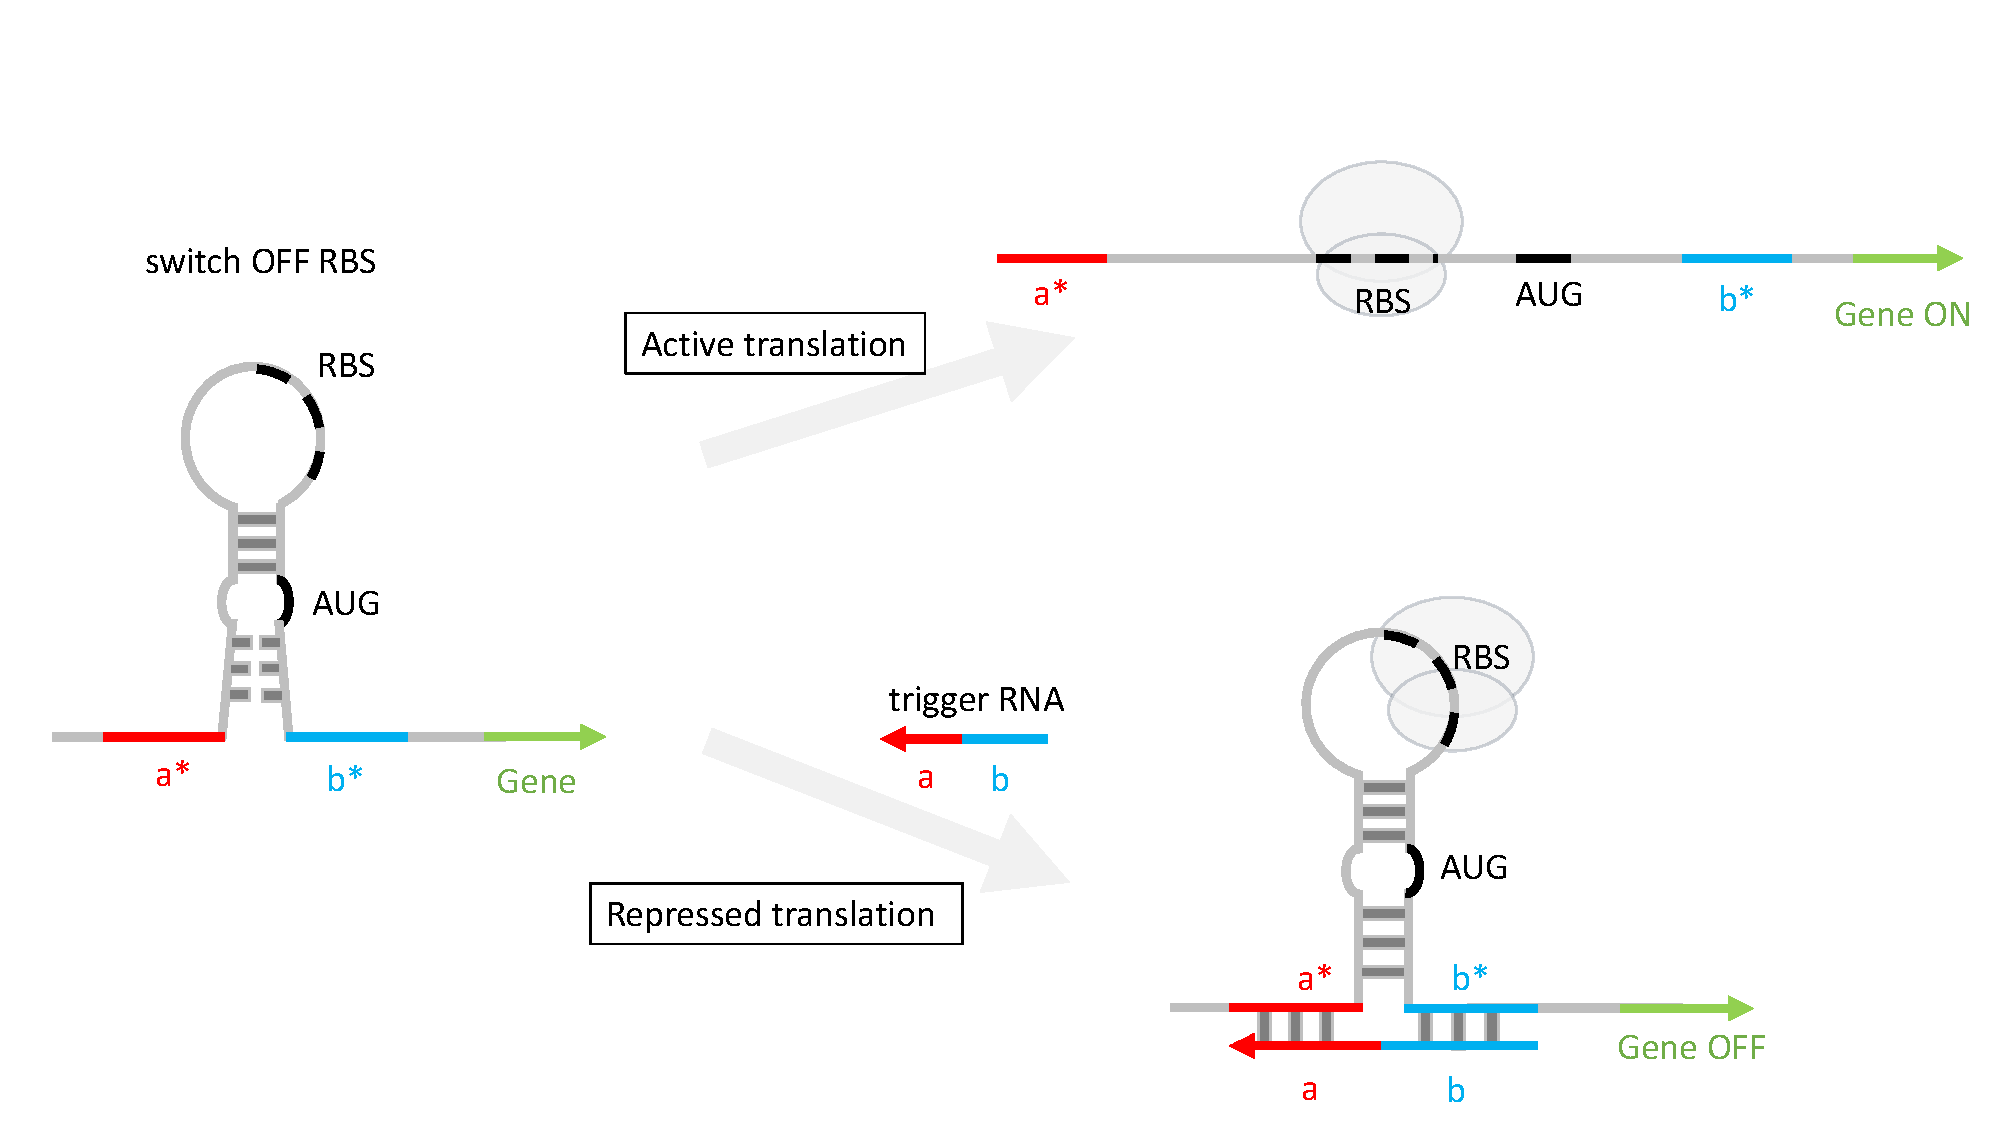
\includegraphics[width=\linewidth]{xor_ribocomputing/switch_off}
        \caption{%
            The unstable hairpin is sealed by 
            the trigger RNA \ce{ab},
            repressing translation.
            %
            Following 
            \cite[\href{https://www.nature.com/articles/s41589-019-0388-1/figures/1}{Fig.~1c}]{Kim2019}.
        }
        \label{f:switch_off_RBS}
    \end{subfigure}
    
    \vspace{1.5\baselineskip}
    
    \begin{subfigure}{\linewidth}
        \centering
        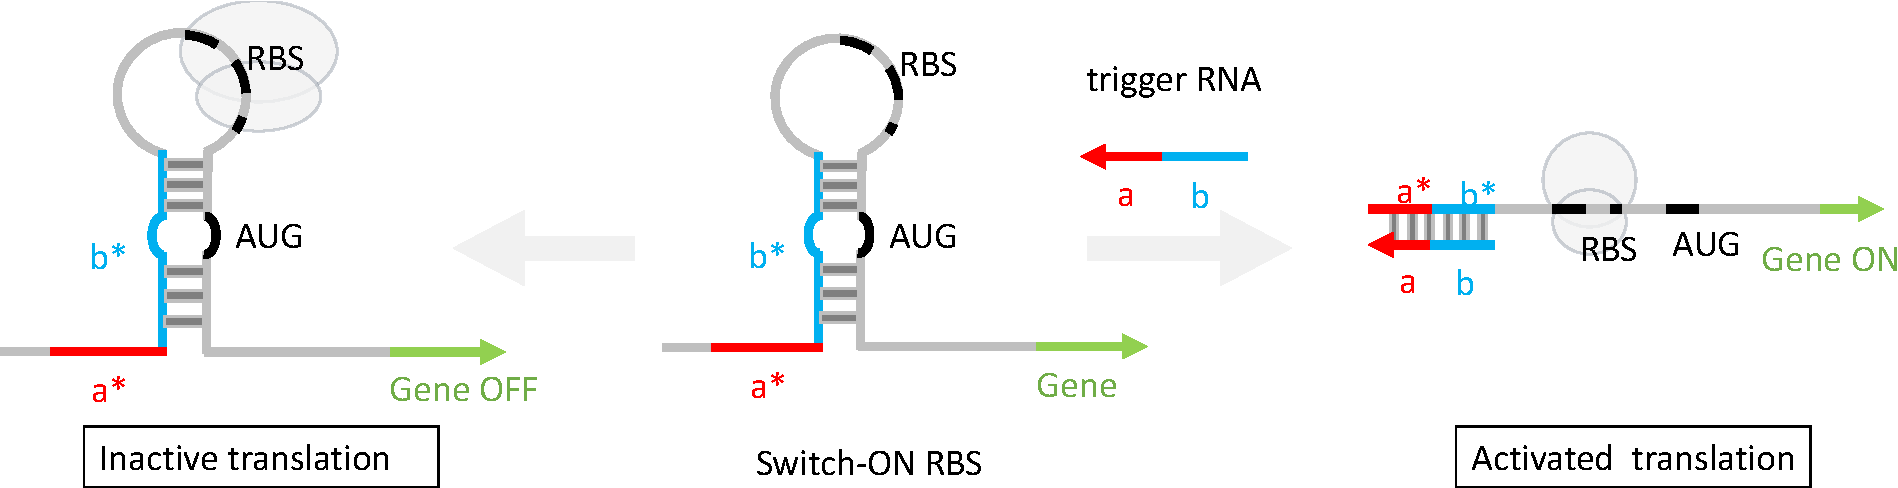
\includegraphics[width=\linewidth]{xor_ribocomputing/switch_on}
        \caption{%
            The stem of the stable hairpin 
            is opened by the trigger RNA \ce{ab}, 
            exposing the RBS for translation. 
            %
            Following 
            \cite[\href{https://www.sciencedirect.com/science/article/pii/S0092867414012896}{Fig.~1b}]{Green2014}.
        }
        \label{f:switch_on_RBS}
    \end{subfigure}
    
    \vspace{1.5\baselineskip}
    
    \begin{subfigure}{\linewidth}
        \centering
        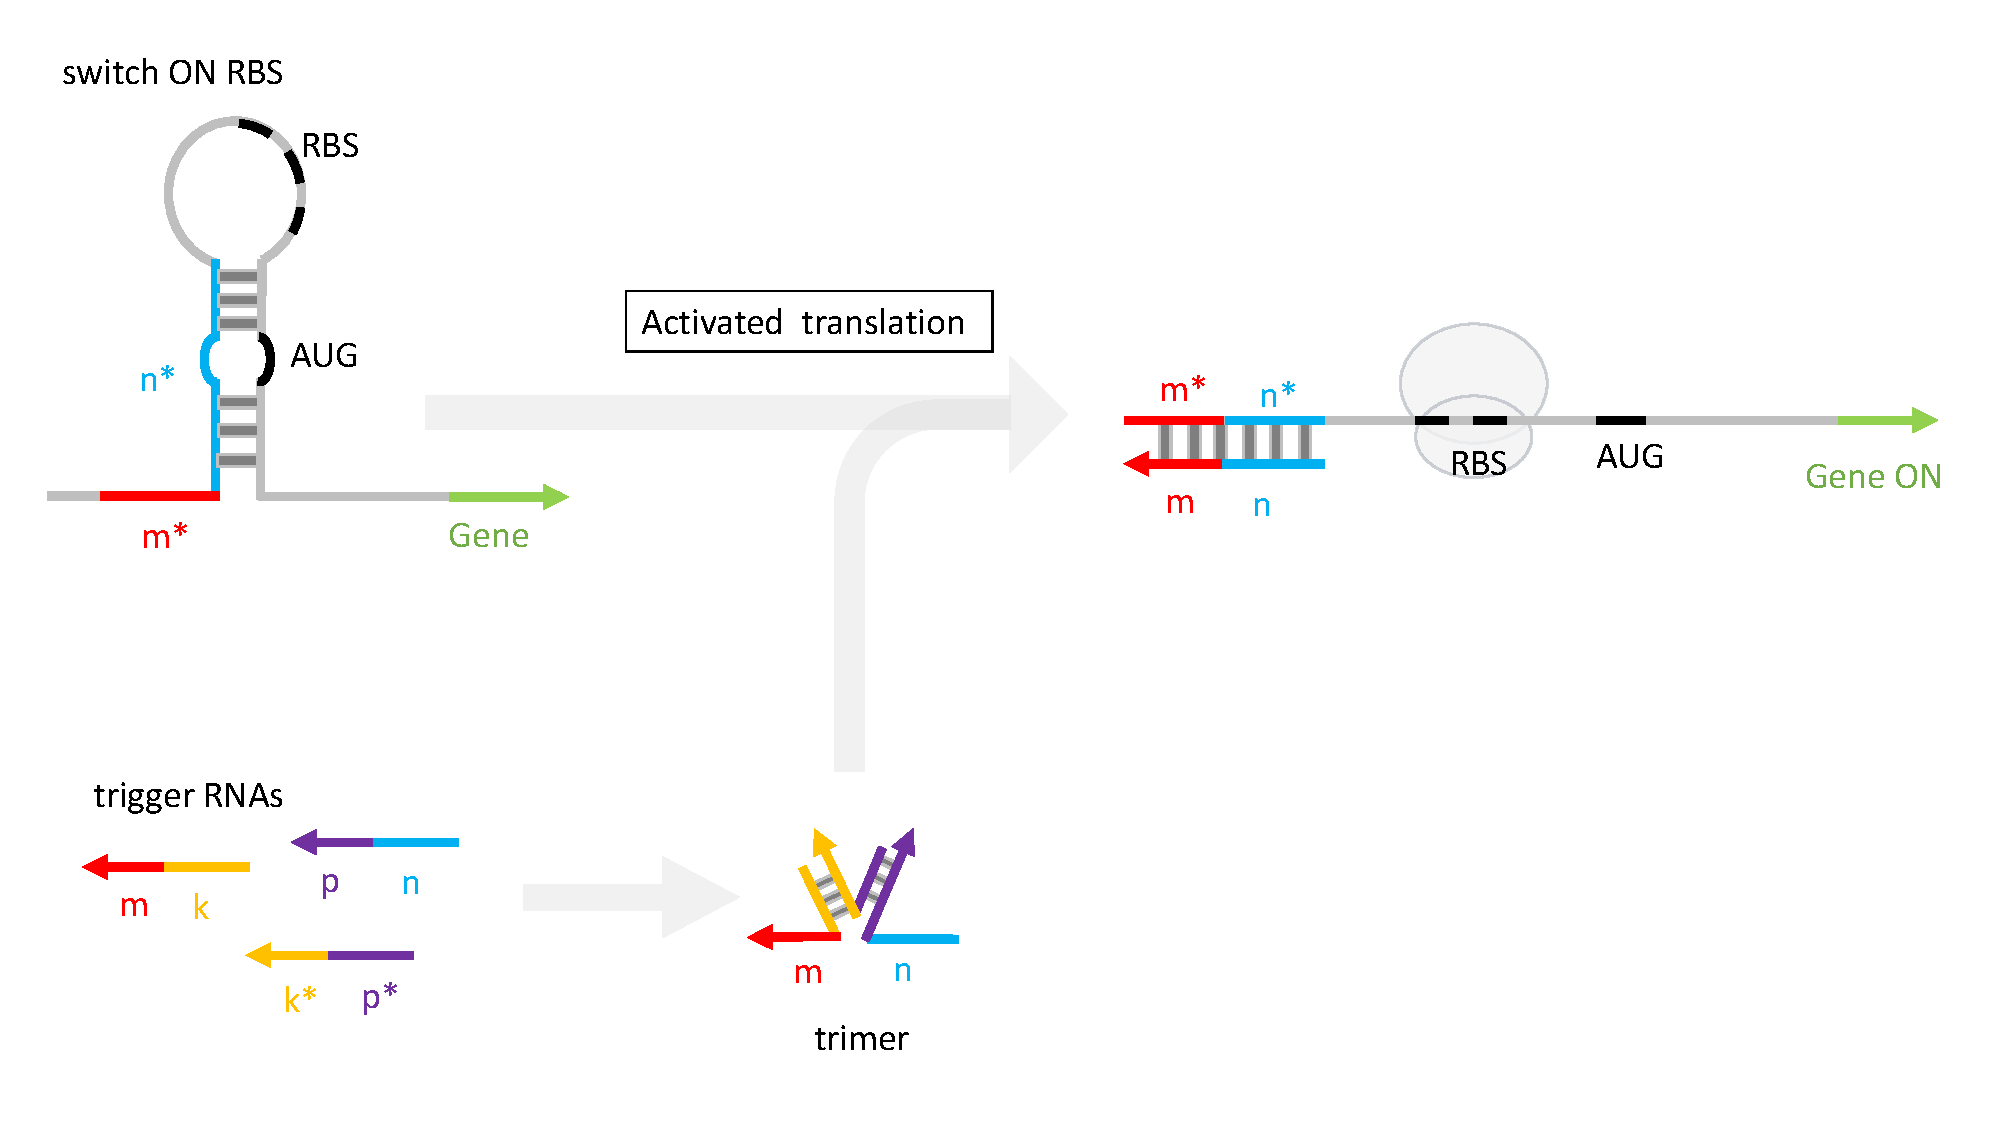
\includegraphics[width=\linewidth]{xor_ribocomputing/3_trigger_rna_on}
        \caption{%
            The co-trigger RNAs form a trimer that switches ON the RBS.
            %
            Following
            \cite[\href{https://www.nature.com/articles/nature23271/figures/3}{Fig.~3a}]{GreenETAL2017}.
        }
        \label{f:3_RNA_on_RBS}
    \end{subfigure}
    
    \caption{%
        Switch-OFF (\ref{f:switch_off_RBS})
        and 
        Switch-ON (\ref{f:switch_on_RBS}) RBS;
        %
        RNAs 3-\AND gate (\ref{f:3_RNA_on_RBS}). 
        %
        Cf.~\S\ref{ss:3xor}/\S\ref{ss:ribocomputing}.
    }
    \label{f:switch_RBS}
\end{figure}



    
    
\begin{figure}
    \centering
    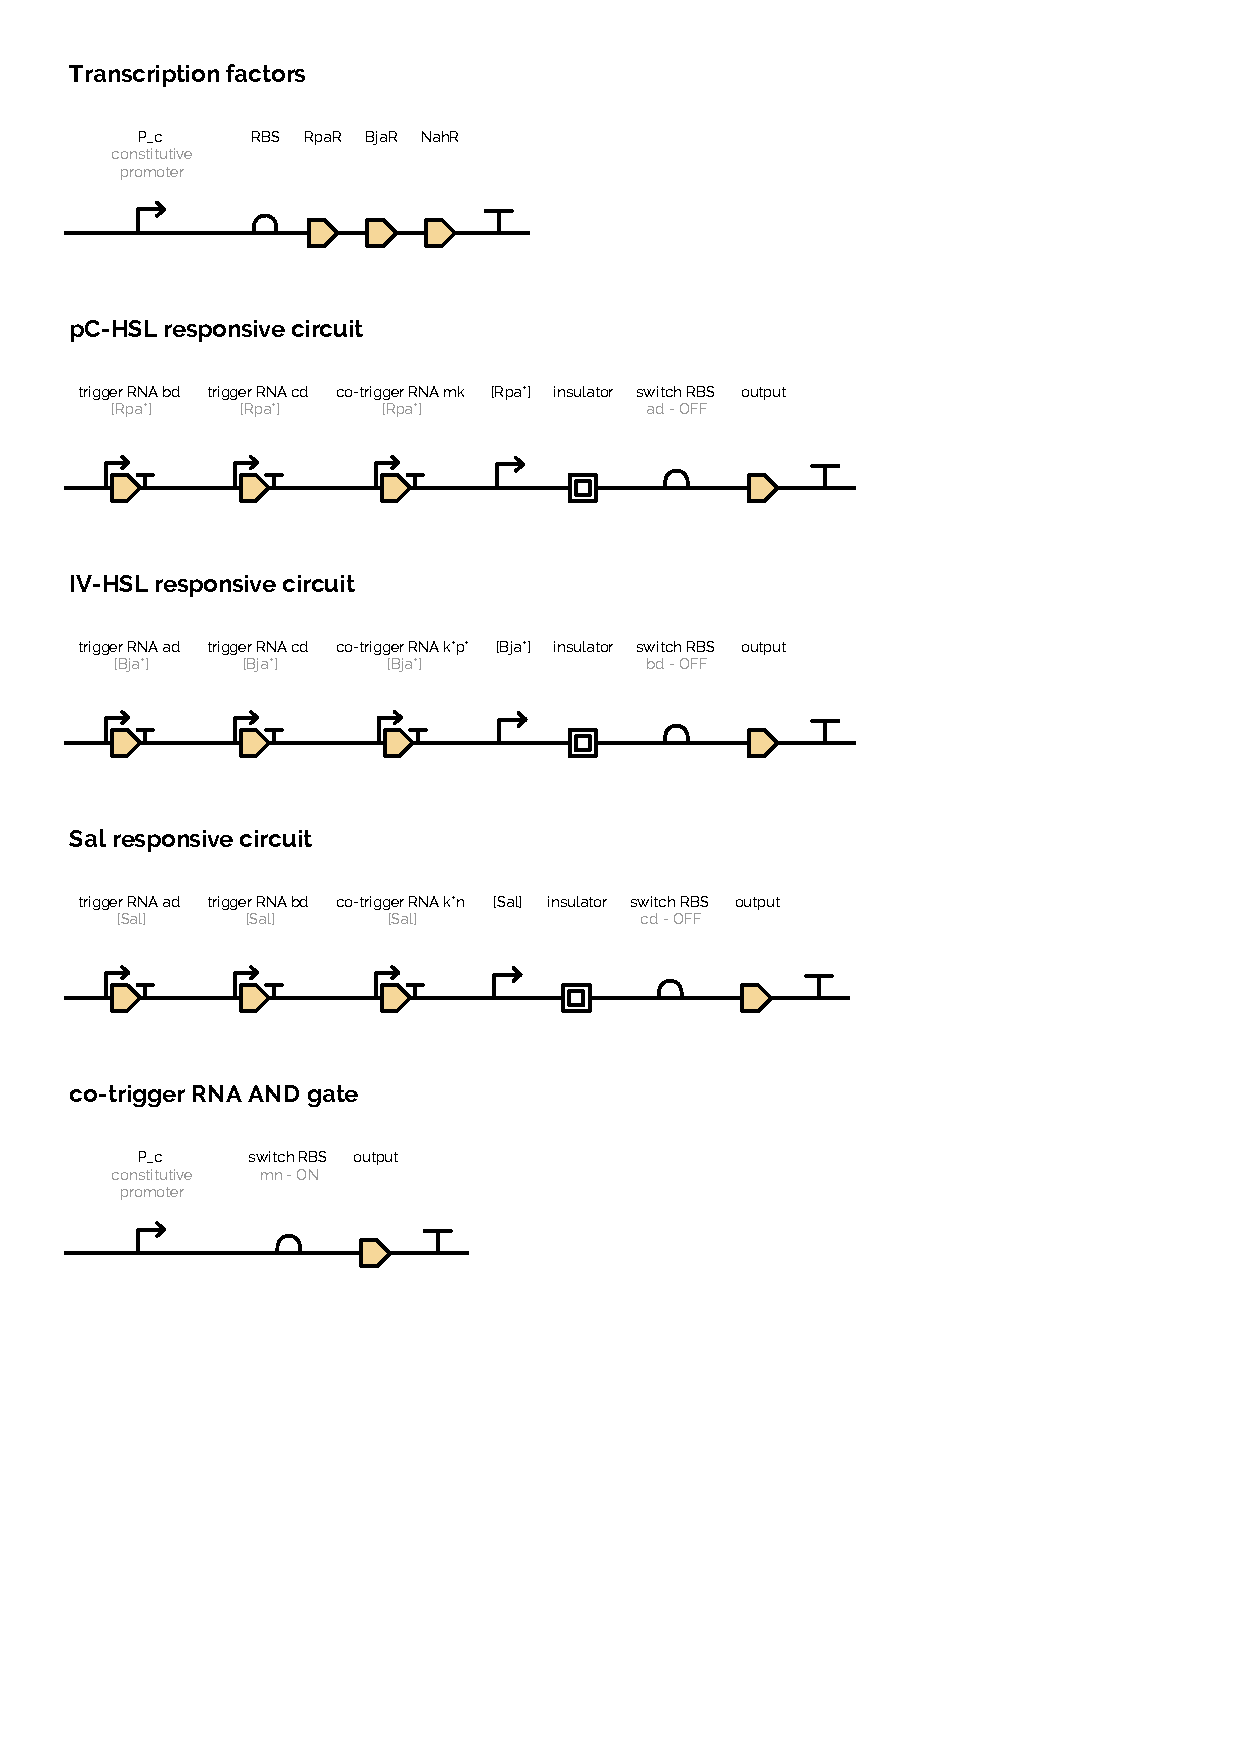
\includegraphics[height=(\textheight-2\baselineskip)]{images/xor_ribocomputing/xor_circuit_plot_2.pdf}
    \caption{Genetic circuits for the 3-input \XOR gate. See \S\ref{ss:3xor}.}
    \label{f:p_construct_xor}
\end{figure}





\subsection{Shelving}

\ra{
The 3-\XOR gate from \S\ref{ss:3xor}
activates or represses translation of an output mRNA.
%
We take this output to be 
the transcription factor \ce{cI^a}
that activates the expression of 
a trigger RNA \ce{Y} with toehold,
which 
in turn triggers the translation of \ce{Xis}.
%
Thus, the presence of \ce{Y} stands for $d_1 = 1$.
}
%
%
%
Now, suppose
\ce{w_B = 1} and \ce{s_1 r_1 c_1 = 101},
in which case \ce{d_1 = 0}.
%
%
Then \ce{Y} is low,
but
around the timepoint when 
\ce{w_B} is turned off
and the inputs begin to change,
\ce{Y} can exhibit a transient bump
(which we observed in some simulations).
%
This can cause production of \ce{Xis}
and 
an unintended \emph{reset}.
%
One way to mitigate this is to condition 
the expression of \ce{Xis}
on \ce{w_B} as well,
which requires \ce{w_B} to go down early
and also tuning of degradation rates.
%
We implemented another, complementary way,
which
is a ``shelf'' (a buffer) for \ce{Y}
that 
%
i)
has high affinity for \ce{Y};
%
ii)
sequesters 
about 
30$\times$EC50${}_\text{\ce{Y}\act\ce{Xis}}$
copies of \ce{Y};
%
iii)
is degraded when \ce{w_A} is on.
%
In this way, 
a transient increase in \ce{Y} is shelved
but a sustained signal 
(while \ce{w_B} is up)
will overflow the shelves and 
allow
translation of \ce{Xis},
cf.~Fig.~\ref{f:symbio-d1-tempo}.
%
%
%
%
As a concrete mechanism
we propose
transcription of 
a repeated complement of \ce{Y},
viz.~%
$
	\signal{\ce{w_A}} \act \protein{AraC^*} \act \promoter{BAD} 
	\act 
	\protein{cI^b} \rep \promoter{cI^b_-} \act
	\ce{[Y^*]^n}
	.
$
%



\section{Simulations}

\subsection{General considerations}

Recall from \S\ref{ss:AmtR}
that 
the dimerized \protein{AmtR} represses \promoter{AmtR},
which we can express as
%
\[
	\ce{2 \protein{AmtR}} + \promoter{AmtR}_\text{active}
	\ce{<=>>}
	\protein{AmtR}_2 \with \promoter{AmtR}
	=
	\text{repressed state}
	.
\]
%
%
In steady state, we have the Hill equation
\[
	\promoter{AmtR}_\text{active}
	& =
	\left(
		1 + 
		(\protein{AmtR} / \text{EC50})^n
	\right)^{-1}
	\promoter{AmtR}_\text{total}
	.
\]
%
%
In case of an activator we use, for example,
\[
	\label{e:Sal}
	%
	\promoter{Sal}_\text{active}
	\ce{=}
	\left(
		1 +
		(\text{EC50} / \signal{Sal})^n
	\right)^{-1}
	\promoter{Sal}_\text{total}
	.
\]
%
%
All species are in units of \emph{molecules}.
%
For simplicity,
we use the above Hill equations
(which, notably, have no baseline term)
for all species with $n = 2$ 
and 
mostly $\text{EC50} = 1$ molecules
(cf.~\S\ref{s:discussion}).
%
%
%
%
%
We simulate production and degradation
such that
typically
about $10$ molecules of output 
from a fully active promoter
correspond to the steady state,
for example
$
	\tfrac{\d}{\d{t}}
	\protein{Output}
	=
	k_+ \promoter{Sal}_\text{active} - k_- \protein{Output}
$
with
$k_+ = 1 \ce{s^{-1}}$
and
$k_- = 0.1 \ce{s^{-1}}$
models 
$\promoter{Sal}_\text{active} \act \protein{Output}$.
%
%
Generally,
we take $0.1$ and $10$ molecules to mean \emph{off} and \emph{on},
respectively.


\TODO{more general considerations?}


\subsection{PlayerA} \label{s:sim:player}

\url{https://github.com/numpde/ibiocomp/tree/main/code/20201231_SymBio_All/PlayerA}

\TODO{on Player A}


%

\begin{figure}[!p]
	\begin{tabular}{cc|cc}
		\multicolumn{2}{c|}{\ce{\#r_1}} & \multicolumn{2}{c}{\ce{\#r_0}}
		%
		\\
		\hline
		%
		\ce{\#w_A} = 0.1 & \ce{\#w_A} = 10 &
		\ce{\#w_A} = 0.1 & \ce{\#w_A} = 10 
		%
		\\
		%
		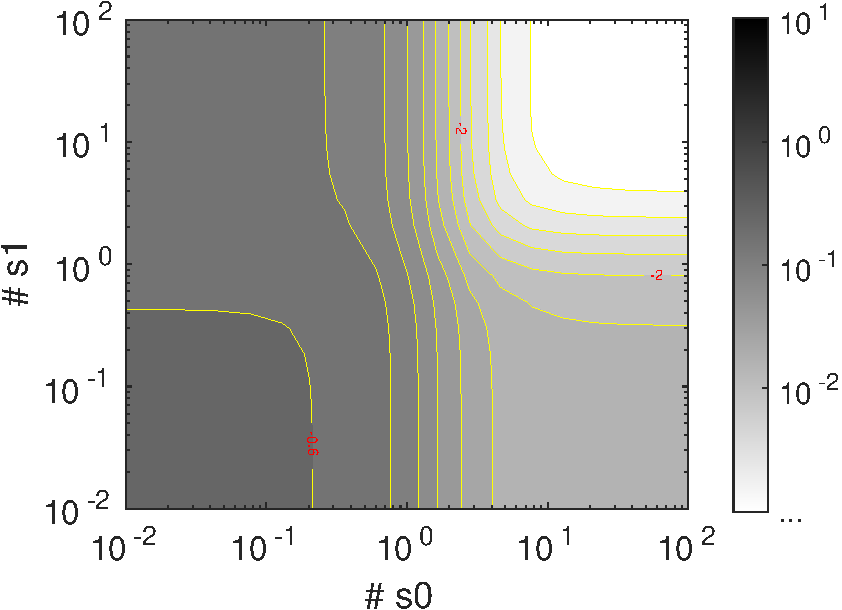
\includegraphics[width=0.22\textwidth]{PlayerA/output/response_r0__wA_in=0.1}
		&
		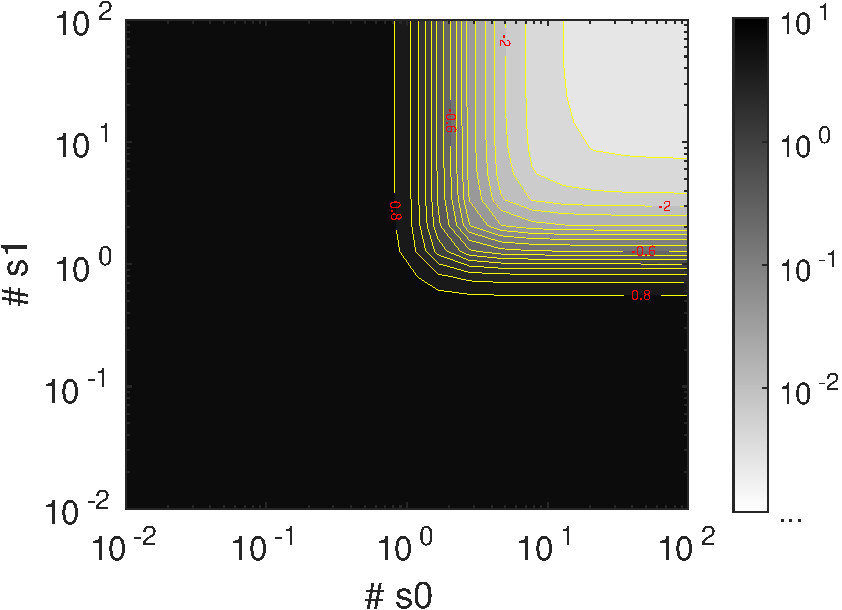
\includegraphics[width=0.22\textwidth]{PlayerA/output/response_r0__wA_in=10}
		&
		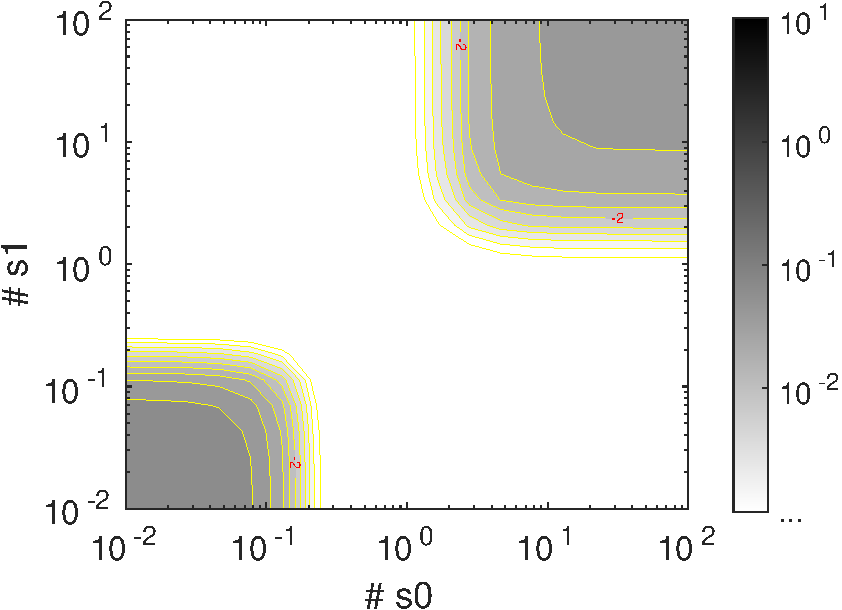
\includegraphics[width=0.22\textwidth]{PlayerA/output/response_r1__wA_in=0.1}
		&
		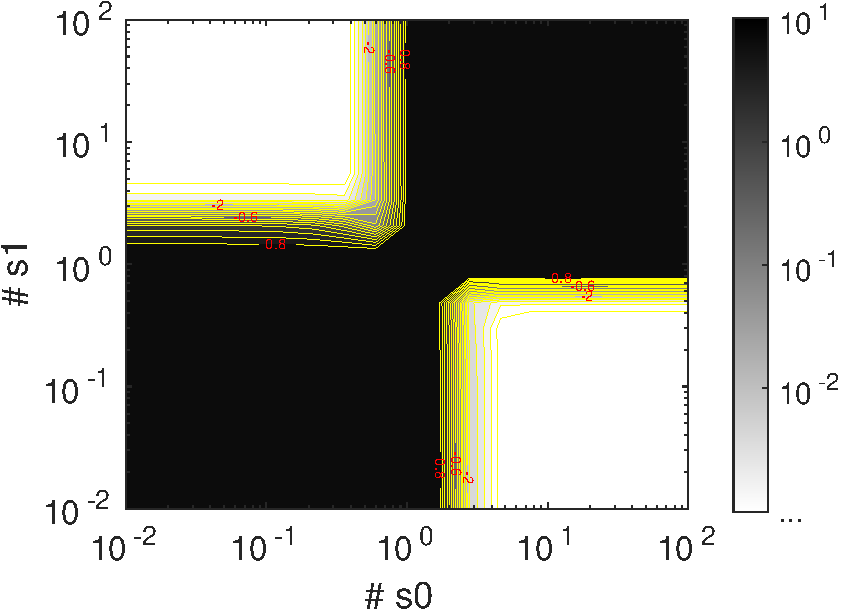
\includegraphics[width=0.22\textwidth]{PlayerA/output/response_r1__wA_in=10}
	\end{tabular}
	%
	\caption{%
		Response surfaces of Player A
		for varying \ce{\#s_1}($\uparrow$) and \ce{\#s_0}($\rightarrow$).
		%
		See \S\ref{s:sim:player}.
		%
		The log-colorbar goes from $10^{-3}$-or-less (white) to $10^1$ (black).
		%
		Yellow contours at $10^t$, $t = 0.8, 0.6, 0.4, \ldots$.
	}
	%
	\label{f:player_response}
\end{figure}





\subsection{Bit 1} \label{s:sim:bit1}

\url{https://github.com/numpde/ibiocomp/tree/main/code/20201231_SymBio_All/Bit1}


\subsubsection*{c2} \label{s:sim:bit1:c2}

\TODO{c2}


\subsubsection*{d1} \label{s:sim:bit1:d1}

\TODO{d1}



\begin{figure}[!p]
	\begin{tabular}{cc|cc}
		\multicolumn{2}{c|}{\ce{\#d_1} with shelving}
		&
		\multicolumn{2}{c}{\ce{\#c_2} with cross-inhibition}
		%
		\\
		\hline
		%
		\ce{\#c_1} = 0.1 & \ce{\#c_1} = 10 &
		\ce{\#c_1} = 0.1 & \ce{\#c_1} = 10 
		%
		\\
		%
		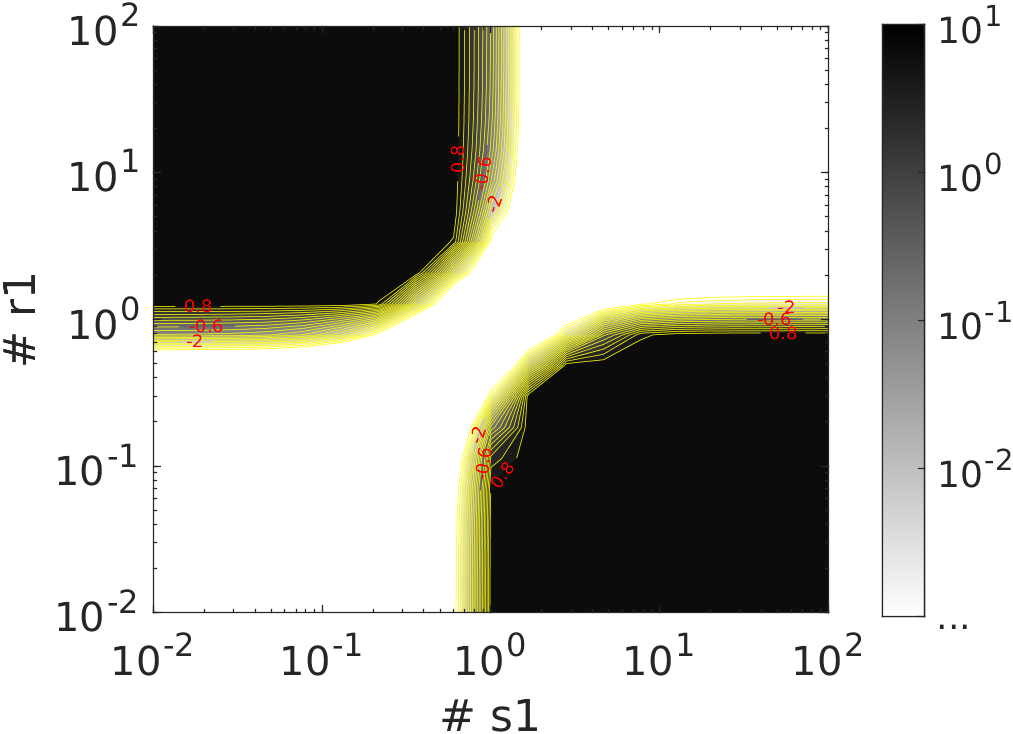
\includegraphics[width=0.22\textwidth]{Bit1/output/response_d1_final__Shelf=1__c1_in=0.1}
		&
		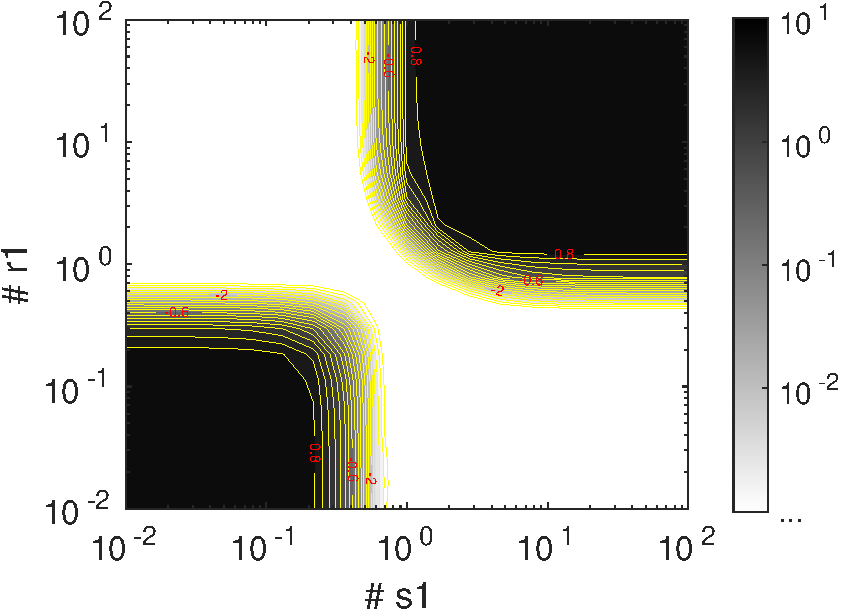
\includegraphics[width=0.22\textwidth]{Bit1/output/response_d1_final__Shelf=1__c1_in=10}
		&
		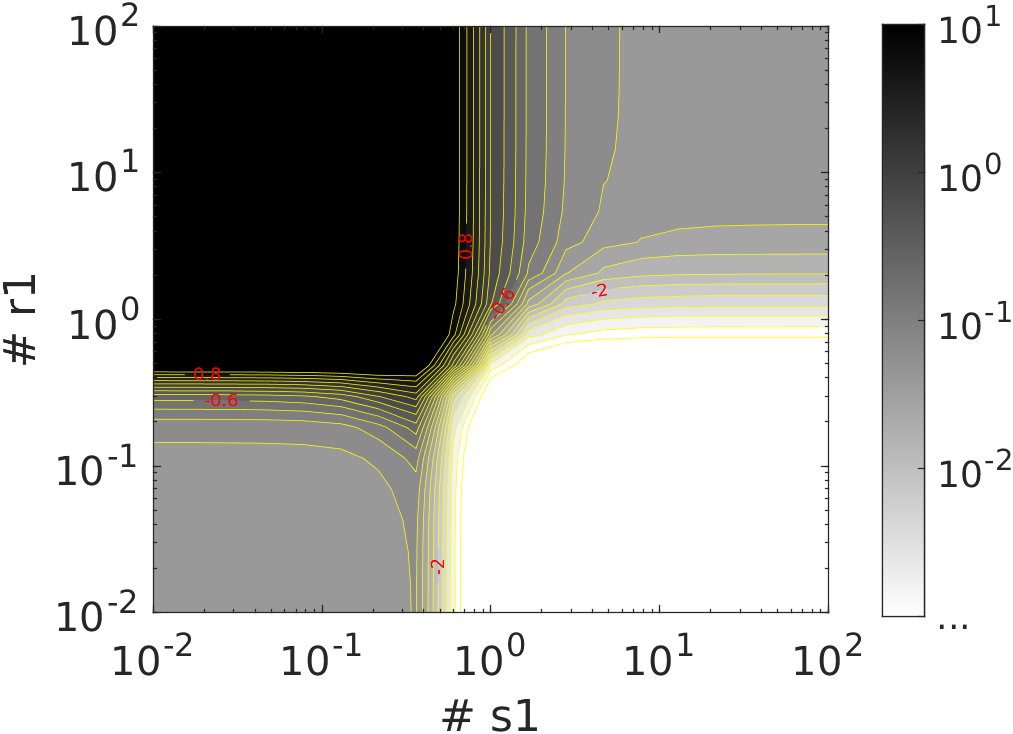
\includegraphics[width=0.22\textwidth]{Bit1/output/response_c2_final__CI=1__c1_in=0.1}
		&
		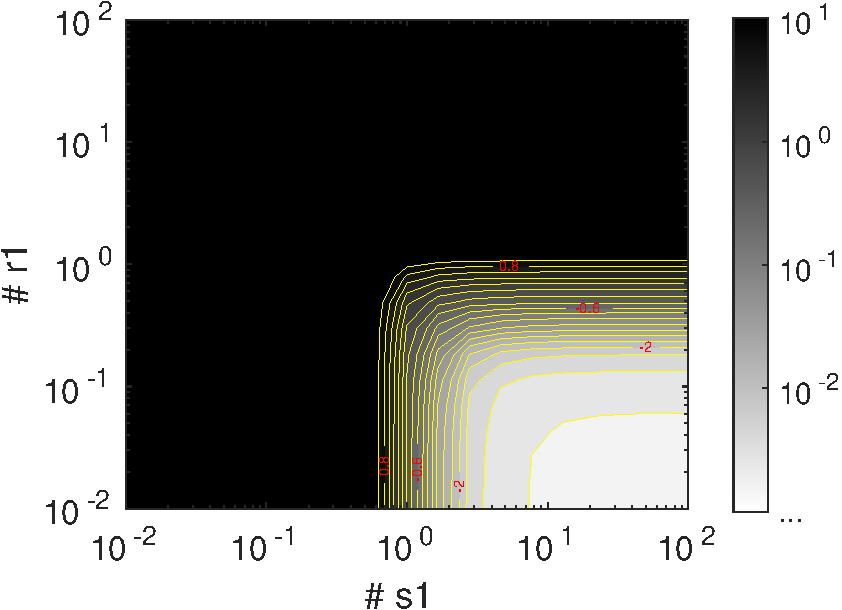
\includegraphics[width=0.22\textwidth]{Bit1/output/response_c2_final__CI=1__c1_in=10}
	\end{tabular}
	
%	\begin{tabular}{cc|cc}
%		\multicolumn{2}{c|}{\ce{\#d_1} without shelving}
%		&
%		\multicolumn{2}{c}{\ce{\#c_2} without cross-inhibition}
%		%
%		\\
%		\hline
%		%
%		\ce{\#c_1} = 0.1 & \ce{\#c_1} = 10 &
%		\ce{\#c_1} = 0.1 & \ce{\#c_1} = 10 
%		%
%		\\
%		%
%		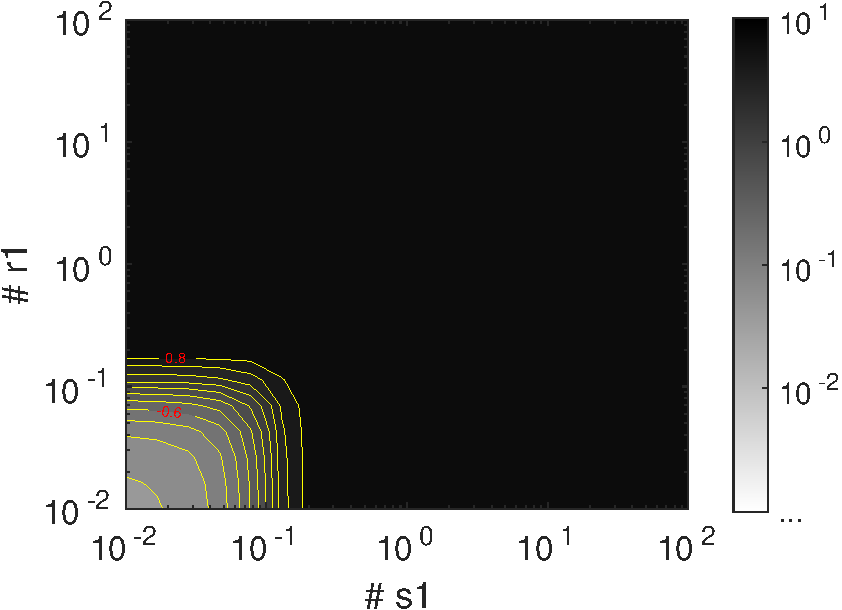
\includegraphics[width=0.22\textwidth]{Bit1/output/response_d1_final__Shelf=0__c1_in=0.1}
%		&
%		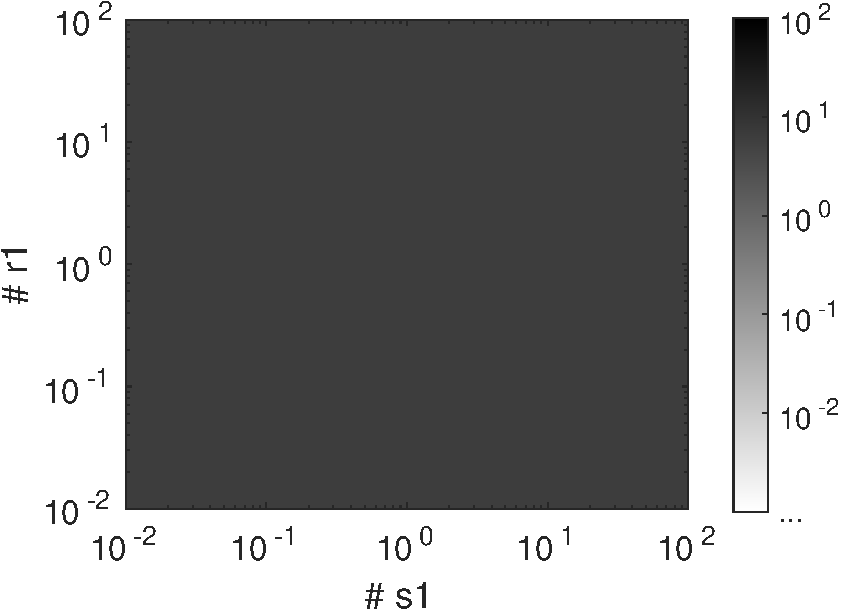
\includegraphics[width=0.22\textwidth]{Bit1/output/response_d1_final__Shelf=0__c1_in=10}
%		&
%		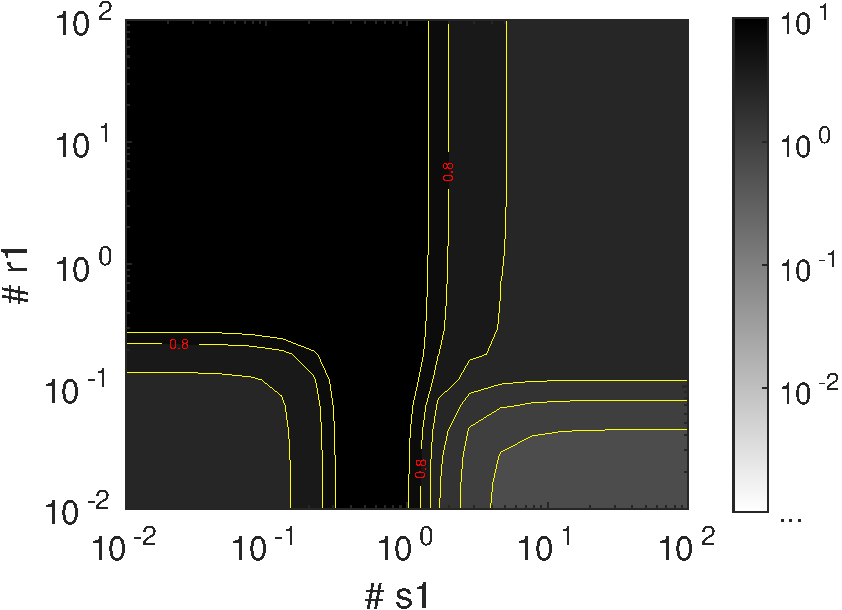
\includegraphics[width=0.22\textwidth]{Bit1/output/response_c2_final__CI=0__c1_in=0.1}
%		&
%		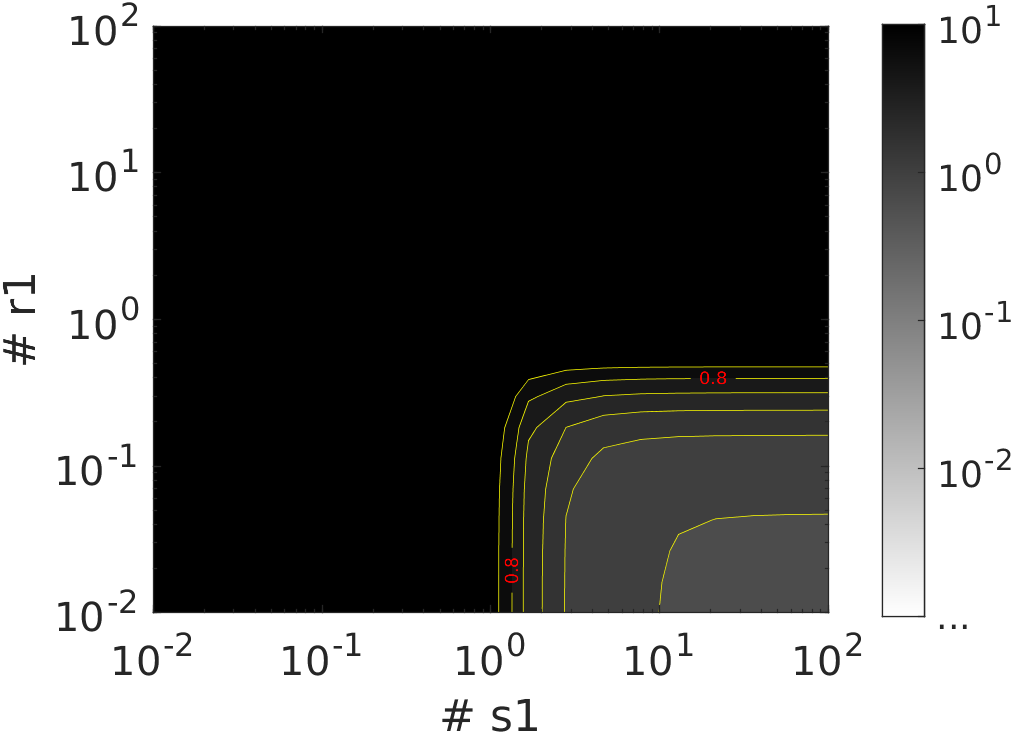
\includegraphics[width=0.22\textwidth]{Bit1/output/response_c2_final__CI=0__c1_in=10}
%	\end{tabular}
	
	\caption{%
		Response of Subtractor A
		for varying \ce{\#r_1}($\uparrow$) and \ce{\#s_1}($\rightarrow$).
		%
		See \S\ref{s:sim:bit1}.
		%
		The output \ce{\#d_1}
		is measured after a compute-, inter- and readout-phase,
		cf.~Fig.~\ref{f:symbio-d1-tempo}.
		%
		The log-colorbar goes from $10^{-3}$-or-less (white) to $10^1$ (black).
		%
		Yellow contours at $10^t$, $t = 0.8, 0.6, 0.4, \ldots$.
	}
	%
	\label{f:sub_response}
\end{figure}

%

\begin{figure}[!p]
    \centering
    %
    \begin{overpic}[width=0.99\textwidth]{Bit1/output/response_d1_tempo__Shelf=1}
    \put (50, 30) {%
    	\scalebox{0.7}{%
    		\begin{tabular}{c|ccc|c}
    		    & \ce{\#s_1} & \ce{\#r_1} & \ce{\#c_1} & $\ce{\#d_1} \approx$
    		    \\
    		    \hline
    		    \ce{B_1} & 10 & 10 & 10 & 0 
    		    \\
    		    \ce{A_1} & {\color{gray}$0.01$} & {\color{gray}$0.01$} & {\color{gray}$0.01$} & 10 
    		    \\
    		    \ce{B_2} & 10 & {\color{gray}$0.01$} & 10 & 0 
    		    \\
    		    \ce{A_2} & {\color{gray}$0.01$} & {\color{gray}$0.01$} & {\color{gray}$0.01$} & 0
    		    \\
    		\end{tabular}
    	}
    }
    \end{overpic}
    %
    \caption{%
        Subtractor A, Bit 1, output \ce{\#d_1}
        across phases \ce{B_1}-\ce{A_1}-\ce{B_2}-\ce{A_2}
        (with interphases).
        %
        The table shows the inputs for each phase.
        %
        We have
        $\#\ce{d_1} \approx 10$ 
        in the recall phase \ce{A_1}
        and
        $\#\ce{d_1} \approx 0$ 
        in \ce{A_2}.
        %
        Observe the slight delay in the rise of Y
        at the beginning of \ce{B_1} while it is being ``shelved'';
        conversely,
        the leakage of Y is ``shelved''
        during \ce{B_2}
        preventing unwanted expression of Xis.
        %
        At the end of \ce{B_2},
		a small deliberate mistiming in signal decay
        leads to a bump in Y 
        that is absorbed by the shelf.
        %
        See also \S\ref{s:sim:bit1:d1}/p.\pageref{s:sim:bit1:d1}.
    }
    %
    \label{f:symbio-d1-tempo}
\end{figure}

%

\section{Discussion} \label{s:discussion}

\TODO{risks}

\begin{itemize}
\item 
    senders and receivers in the same cell
\item
    In reality,
    the EC50 of the signals
    varies over several orders of magnitude
    \cite[SM:Fig.~8]{DuETAL2020}.
\item
    \citet[SM:p.10]{NielsenETAL2016}
    reported
    $n = 1.6$ for an insulated AmtR
    (with a certain RBS),
    and higher coefficients for
    some other transcription factors.
\item
    Timing could be an issue.
\end{itemize}


\section{Acknowledgments}

\TODO{ack}



%%% BIBLIOGRAPHY %%%
\clearpage

\footnotesize
\bibliographystyle{apalike}
\bibliography{refs}
\normalsize




\clearpage


\section*{Appendix}


\subsection{Subtractor module}

Fig.~\ref{f:logical-subtractor01} 
shows the principles of
the Subtractor module (bit 0 and bit 1),
but our implementation
differs in the details.
%
In particular, we use a reversible recombinase
for the memory module, see \S\ref{ss:memory}/p.\pageref{ss:memory}.

% https://www.circuit-diagram.org/editor/c/075f8cf9d084400b94f1384cc1c3ba96
\begin{figure}[phbt]
\centering
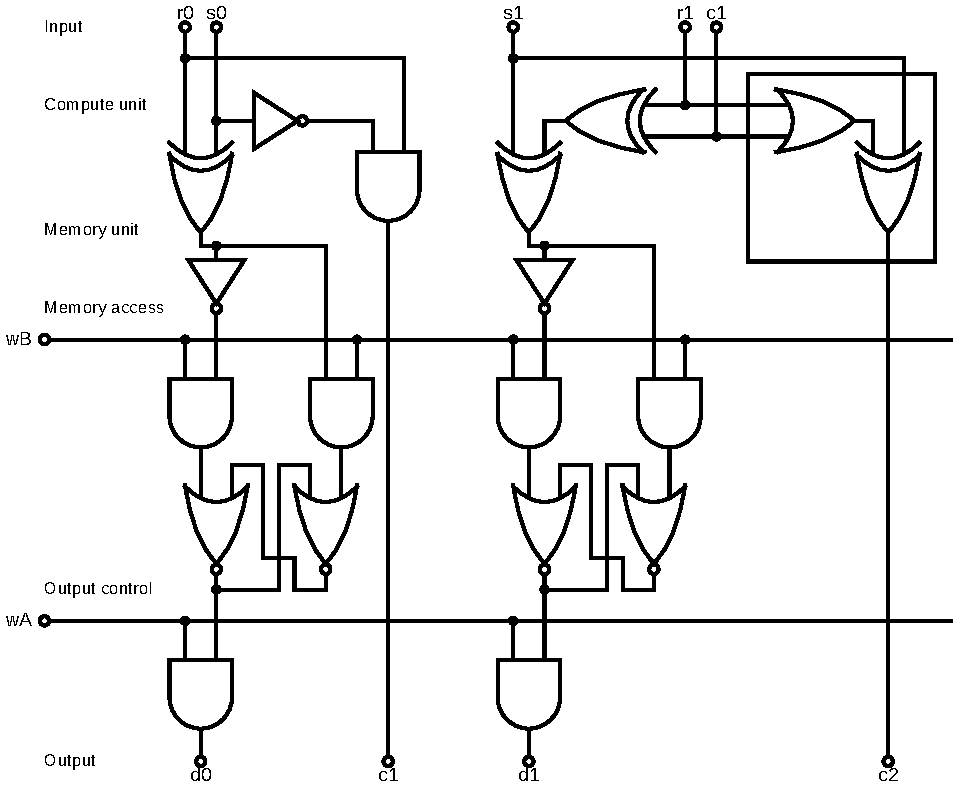
\includegraphics[width=0.9\linewidth]{circuits/Logical-HalfSubtractor0.svg.pdf}
%
\caption{%
Bit~0 and Bit~1
of
Subtractor~A.
%
The result of the compute unit is written to the memory unit
(e.g.~a bistable switch)
when the signal \ce{w_B} is present.
%
The value of the memory unit is
forwarded to the output
when the signal \ce{w_A} is present.
}
\label{f:logical-subtractor01}
\end{figure}



\subsection{Phases}

\begin{table}[hpbt]
    \centering
    %
    % Table made with
    % https://deepnote.com/project/998c51eb-bb3f-4a0f-88e3-c8b50d4d678a#%2Ft_phases.ipynb
    %
    \begin{tabular}{l||cc|ccc|ccc|ccc|cc}
    {} &      \ce{r_0} &      \ce{r_1} &    \ce{s_0} &      \ce{d_0} &      \ce{c_1} &      \ce{s_1} & \ce{d_1} &      \ce{c_2} &    \ce{s_2} &      \ce{d_2} &      \ce{c_3} &    \ce{s_3} &      \ce{d_3} \\ 
    \hline
    1 &  $\downarrow$ &  $\downarrow$ &  $\uparrow$ &               &               &    $\uparrow$ &          &               &             &               &               &             &               \\ 
    \hline
    2 &    $\uparrow$ &               &  $\uparrow$ &  $\downarrow$ &  $\downarrow$ &               &          &               &             &               &               &             &               \\ 
    \hline
    3 &               &    $\uparrow$ &             &               &    $\uparrow$ &  $\downarrow$ &          &  $\downarrow$ &             &               &               &             &               \\ 
    \hline
    4 &               &               &             &               &               &               &          &    $\uparrow$ &  $\uparrow$ &  $\downarrow$ &  $\downarrow$ &             &               \\ 
    \hline
    5 &               &               &             &               &               &               &          &               &             &               &    $\uparrow$ &  $\uparrow$ &  $\downarrow$ \\ 
    \hline
    \end{tabular}
    %
    %
    \caption{%
        Substeps of each phase A/B.
        Arrows: emit ($\uparrow$) and compute ($\downarrow$).
    }
    \label{t:substeps}
\end{table}







\clearpage



\section*{Final TODOs}

\TODO{spacing of act and rep}

\TODO{check that Table \ref{t:signals} is correct}

\TODO{stars}


\clearpage

\SHOWTODOS




\leavevmode\vfill{\tiny\color{lightgray}\hfill{\DTMnow}}
\end{document}





